
\documentclass[../main]{subfiles}
\ifSubfilesClassLoaded{
    \dominitoc
    \tableofcontentsfile
}{}
\begin{document}
%\graphicspath{{\subfix{/02-Architectures/figures}}}
\graphicspath{{./figures},{02-Architectures/figures}}
\chapter{Architectures de cartes auto-organisatrices}
\minitoc


% Nous avons établi qu'une piste de recherche pour la construction d'algorithmes d'apprentissage passe par l'assemblage d'éléments existants comme modules d'un système, nous cherchons ainsi dans cette thèse à définir un modèle d'architecture d'apprentissage modulaire, comportant des rétroactions apportant un aspect dynamique a ce système. 
Nous nous concentrerons dans cette thèse sur la création d'architectures de cartes auto-organisatrices ou SOM (\emph{Self-Organizing Maps}) comme modules d'une architecture décentralisée.
Les cartes auto-organisatrices et notamment le modèle de Kohonen sont largement utilisées en tant qu'algorithme d'apprentissage non supervisé sur diverses applications, notamment la réduction de dimension et la visualisation de données. Cependant, peu de travaux ont exploré l'idée de les assembler en architecture comportant des rétroactions, formant ainsi un système dynamique. 
L'aspect bio-inspiré des cartes de Kohonen et la présence de motifs auto-organisés motivent pourtant cet axe d'utilisation en tant que système dynamique, motivations que nous présentons dans ce premier chapitre.

Kohonen écrivait par exemple dans son livre à propos des enjeux des cartes de Kohonen en 1995:
\begin{quote}
Un objectif à long terme de l'auto-organisation est de créer des systèmes autonomes dont les éléments se contrôlent mutuellement et apprennent les uns des autres. De tels éléments de contrôle peuvent être implémentés par des SOMs spécifiques; le problème principal est alors l'interface, en particulier la mise à l'échelle automatique des signaux d'interconnexion entre les modules et la collecte de signaux pertinents comme interface entre les modules. Nous laisserons cette idée aux recherches futures.
\cite{Kohonen1995SelfOrganizingM}
\end{quote}

% Systems of SOMs. A far-reaching goal in self-organization is to create
% autonomous systems, the parts of which control each other and learn from
% each other. Such control structures may be implemented by special SOMs;
% the main problem thereby is the interface, especially automatic scaling of
% interconnecting signals between the modules, and picking up relevant signals
% to interfaces between modules. We shall leave this idea for future research. 

L'idée de trouver de nouveaux paradigmes de calculs non conventionnels dans les SOMs à l'aide de leur assemblage en structure modulaire dynamique rejoint l'idée de Kohonen sur les systèmes autonomes. 
Il soulève la question de l'interface entre les modules, qui sera centrale dans notre construction. 
Le but de cette thèse est ainsi d'une part, de proposer un modèle de carte qui puisse être utilisée en tant que module et de définir l'interface entre modules et d'en extraire des comportements de calcul en émergeant. 
Avant toute chose, nous pouvons chercher des éléments de réponse à ces deux questions en étudiant les travaux traitant des architectures de cartes de Kohonen ou plus généralement de réseaux d'apprentissage utilisant des règles d'auto-organisation dans leur évolution. Cela nous permettra de privilégier un type d'interface au regard des travaux existants et d'émettre des hypothèses quant aux comportements attendus de l'architecture que nous proposerons.

Nous présentons ainsi dans ce chapitre le modèle général d'une carte de Kohonen et ses comportements de base; notre modèle sera ensuite décrit plus en détail au chapitre~\ref{chap:modele}.
Nous passons ensuite en revue différentes architectures de SOM proposées dans la littérature. 
Nous analyserons notamment comment la structure d'une architecture définit le type d'apprentissage effectué par un système. Nous comparerons aussi le choix du modèle d'interfaces entre cartes.
A l'issue de ce chapitre, nous aurons une vue d'ensemble organisée de différents modèles d'architectures de SOMs existantes et définirons ou se place le modèle que nous étudierons.
A la lumière des résultats des différents travaux, nous proposerons des hypothèses sur les comportements que nous pouvons attendre de notre modèle d'architecture. 
Ces hypothèses motivent les expériences conduites dans la suite de cette thèse. 

\section{Les cartes auto-organisatrices de Kohonen comme modules d'une architecture}\label{sec:som001}

Le modèle de cartes auto-organisatrice a été initialement développé par Kohonen \cite{Kohonen1982}~; nous utiliserons ainsi les termes cartes de Kohonen et SOM de façon équivalente pour désigner ce modèle initial.
De nombreux modèles dérivés ont ensuite été développés à partir de ce modèle initial, sur diverses applications.
Nous présentons dans cette section le modèle de carte de Kohonen et détaillons les possibilités qu'il offre en tant que module d'une architecture. 

\subsection{Carte de Kohonen classique}

Une carte de Kohonen est un algorithme de quantification vectorielle. Le but de la quantification vectorielle est de représenter un ensemble de données d'entrées issues d'un espace $\mathcal{D}$ en un nombre fini de vecteurs de l'espace d'entrée, les prototypes. Dans une SOM, ces prototypes sont disposés sur les n\oe{}uds d'un graphe, en général une grille en deux dimensions.
Les n\oe{}uds du graphe possèdent alors chacun un prototype et sont \emph{indexés}, par un réel ou un vecteur en deux dimensions lorsque que la carte est une grille.
Cette indexation et le format de graphe permet de définir une distance dans la carte et une notion de voisinage entre n\oe{}uds.
Nous appellerons carte de Kohonen le graphe assorti de ses prototypes.

Au début de l'apprentissage, les prototypes prennent une valeur aléatoire dans l'espace d'entrée. 
L'apprentissage est ensuite réalisé en trois étapes~:
\begin{enumerate}
\item Une entrée $\inpx$ est présentée à la carte.
\item Le n\oe{}ud ayant le prototype le plus proche de $\inpx$ selon une distance $d$ est choisie comme \emph{Best Matching Unit} (BMU) de la carte. Son index est noté $\bmu$. La distance $d$ généralement utilisée est la distance euclidienne.
\item Le prototype de la BMU est déplacé vers l'entrée $\inpx$, ainsi que les prototypes des n\oe{}uds voisins de $\bmu$ dans un voisinage défini à l'avance. On peut interpréter cette étape comme le déplacement d'une zone de la carte centrée en $\bmu$. Des exemples de voisinages sont ainsi indiquées en figure \ref{fig:topo}. Ce voisinage est défini par une fonction de voisinage dans l'algorithme qui dépend de la distance d'un n\oe{}ud au BMU et associe à chaque n\oe{}ud un coefficient multiplicatif pour la mise à jour des poids. Cette fonction est maximale à la position du BMU et décroissante autour de cette position. Il s'agira par exemple d'une fonction rectangulaire, triangle ou gaussienne.
\end{enumerate}

L'algorithme de Kohonen repose donc à la fois sur un mécanisme de compétition, avec la sélection de la BMU de la carte et un processus de coopération avec le déplacement des unités voisines de la BMU.
Toutes les données d'entrées sont tirées dans un même espace $\mathcal{D}$. L'utilisation de distances est la version originale de l'algorithme de Kohonen; elle est remplacée dans de nombreux modèles de cartes par le calcul d'une fonction d'activité liant les poids des n\oe{}uds et les entrées. 


Le processus de mise à jour des poids d'une carte de Kohonen se traduit visuellement par un dépliement de la carte dans l'espace d'entrée. On parlera donc de \emph{dépliement} d'une carte lorsque qu'on parle d'apprentissage. Ce dépliement est représenté en figures \ref{fig:som2d} et \ref{fig:som1d} pour des exemples de cartes en une et deux dimensions, se dépliant sur des données en deux dimensions. On observe d'ailleurs que les valeurs des poids à l'issue de l'apprentissage correspondent aux centres des cellules de Voronoï de l'espace d'entrée.
A la fin de l'apprentissage, la carte conserve la structure topologique des entrées:
\begin{itemize}
\item Elle conserve les distances~: deux prototypes ayant une distance proche dans la carte seront également proches selon la distance définie dans l'espace d'entrée. On observe donc une continuité des valeurs des poids au sein de la carte.
\item Elle conserve les densités. Une zone dense de $\mathcal{D}$ aura plus d'unités correspondant à cette zone de valeurs dans la carte qu'une zone moins dense.
\end{itemize}
La figure \ref{fig:SOM} présente par exemple le dépliement d'une carte sur des imagettes MNIST.
Par son aspect ordonné, une carte est une représentation en faible dimension d'un espace d'entrée de grande dimension. 

%Les cartes de Kohonen sont souvent utilisées en pratique pour visualiser des données de grande dimension et faire du \emph{clustering}. 

% La carte de Kohonen est d'inspiration biologique. Le but premier de Kohonen était de développer un modèle informatique inspiré de l'organisation spatiale des neurones dans le cortex humain, dont un exemple est présenté en figure~\ref{fig:v1}. Il s'est notamment inspiré de l'organisation du cortex en colonnes corticales, ensemble de neurones réagissant à un même stimulus.

% \draft{
% (Kohonen book 1995)
% In an attempt to implement a learning principle that would
% work reliably in practice, effectively creating globally ordered maps of various
% sensory features onto a layered neural network, this author formalized the
% self-organizing process in 1981 and 1982 into an algorithmic form that is
% now being called the Self-Organizing (Feature) Map (SOM) [2.27 -29J. In the
% pure form, the SOM defines an "elastic net" of points (parameter, reference,
% or codebook vectors) that are fitted to the input signal space to approximate
% its density function in an ordered way. The main applications of the SOM
% are thus in the visualization of complex data in a two-dimensional display,
% and creation of abstractions like in many clustering techniques.

% Motivations de Kohonen: capacité des régions du cerveau à s'auto organiser. Note que certes il doit y avoir un prédetermination génétique, mais qu'on observe une réorganisation des mapping lors de déficiences par ex. 

% find abstract self-
% organizing processes in which maps resembling the brain maps are formed,
% whereas it is of less interest whether the maps are formed by evolution, post-
% natal growth, or learning.

% }

\begin{figure}
\centering
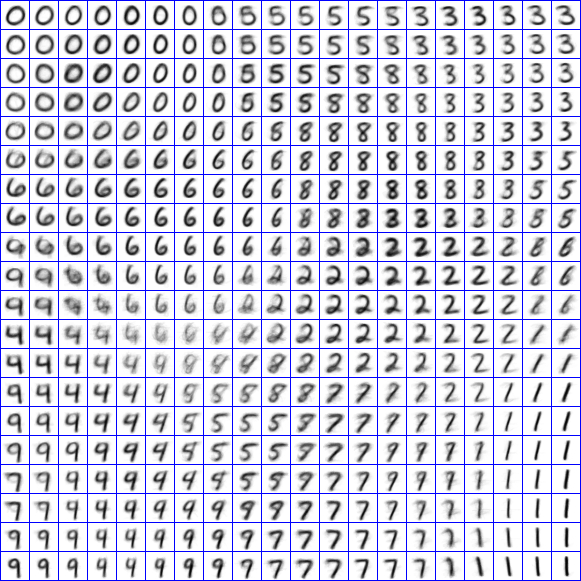
\includegraphics[width=0.5\textwidth]{digits.jpg}
\caption{Représentation de la base de données MNIST, images de chiffres écrits à main levées, par une SOM en deux dimensions. Une continuité est observée dans la forme des images lorsqu'on se déplace dans la carte~: le $0$ se transforme en $6$, etc.}
\label{fig:SOM}
\end{figure}

\subsection{Aspect topologique de la carte de Kohonen}

La carte de Kohonen se distingue d'autres algorithmes de quantification vectorielle par la topologie introduite par la carte dans l'ensemble des prototypes. Cette topologie dépend du voisinage utilisé par l'algorithme et de la dimension du support de la carte.
La plupart des implémentations de SOMs de la littérature utilisent comme support une grille en deux dimensions. L'indexation des n\oe{}uds est alors un ensemble de positions 2D.

En théorie, les cartes peuvent être une dimension (ligne), deux dimensions (grilles), ou de dimensions plus grandes. Les cartes peuvent aussi être des graphes de forme plus variable. En pratique, les grilles deux dimensions sont les plus couramment utilisées. Elles permettent d'effectuer une réduction de dimension, tout en étant facile à visualiser sur un écran. Les cartes de dimensions supérieures sont très rarement utilisées dans la littérature. Le coût de l'algorithme d'apprentissage dépend en effet du nombre de neurones, et celui-ci augmente exponentiellement lorsqu'on augmente la dimension d'une carte de Kohonen. Les calculs deviennent alors rapidement coûteux.
Les cartes une dimension sont quant à elles limitées en termes de représentation des données et sont donc rarement utilisées en pratique. Cependant, elles se prêtent mieux à la représentation graphique que les cartes 2D.
%Les calculs et l'organisation générés par l'algorithme de Kohonen sont assez complexes avec des cartes en une dimension. 
Les travaux conduits en \cite{cottrell_theoretical_2016,fort_soms_2006} apportent par exemple une formalisation mathématique de l'algorithme de Kohonen et prouvent la convergence de cartes une dimension. Les auteurs se heurtent cependant à la preuve de convergence pour des cartes en deux dimensions. Donc, les processus intervenant dans des cartes 1D sont déjà mathématiquement difficiles à formaliser, difficulté qui augmente fortement avec les dimensions.
L'étude des cartes 1D a ainsi l'intérêt d'envisager un modèle simplifié dans le cadre de développement d'un nouveau modèle de SOM, ce que nous chercherons à faire dans cette thèse, avant de proposer une extension aux cartes 2D.

Les cartes de forme autre que des grilles 1D ou 2D sont moins couramment utilisées, mais peuvent avoir des avantages. Ainsi, des cartes structurées en arbre telles que développées en~\cite{koikkalainen_self-organizing_1990} permettant une recherche de BMU structurée. Certains modèles construisent une carte de Kohonen en ajoutant des n\oe{}uds au fur et à mesure de l'apprentissage, générant une carte de Kohonen sous forme d'un graphe construit par l'algorithme, par exemple en~\cite{alahakoon_dynamic_2000, yamaguchi_adaptive_2010}.

\begin{figure}
\centering
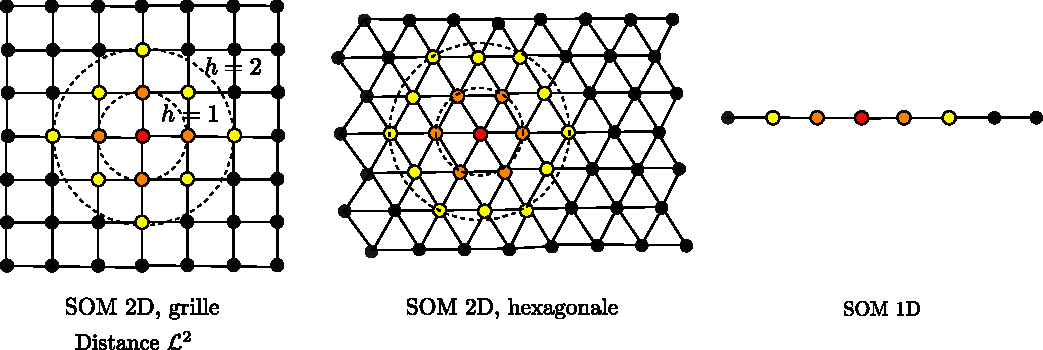
\includegraphics[width=0.8\textwidth]{soms_topologies}
\caption{Exemples de connexions dans le graphe support d'une SOM. Deux n\oe{}uds connectés sont ici à une distance de une unité dans la carte.
Les SOM en deux dimensions sont les plus communément utilisées dans la littérature, sous forme d'une grille ou d'une grille hexagonale. Les SOM une dimension sont également utilisées. \label{fig:topo}}

\end{figure}

\begin{figure}
\centering
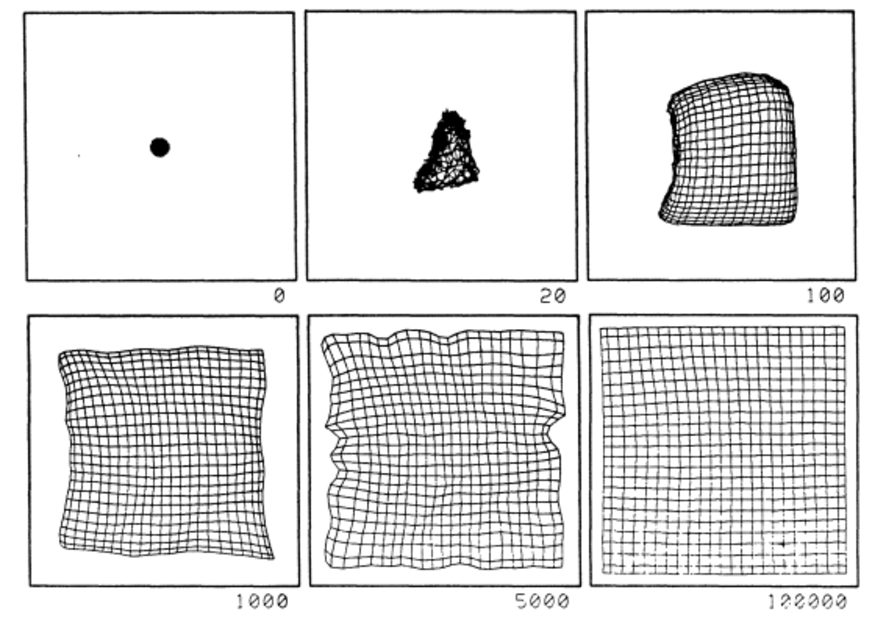
\includegraphics[width=0.7\textwidth]{som2d}
\caption{Dépliement d'une SOM 2D sur des données dans le plan $[0,1]^2$, tiré de~\cite{Kohonen1995SelfOrganizingM} \label{fig:som2d}}

\end{figure}

\begin{figure}
\centering
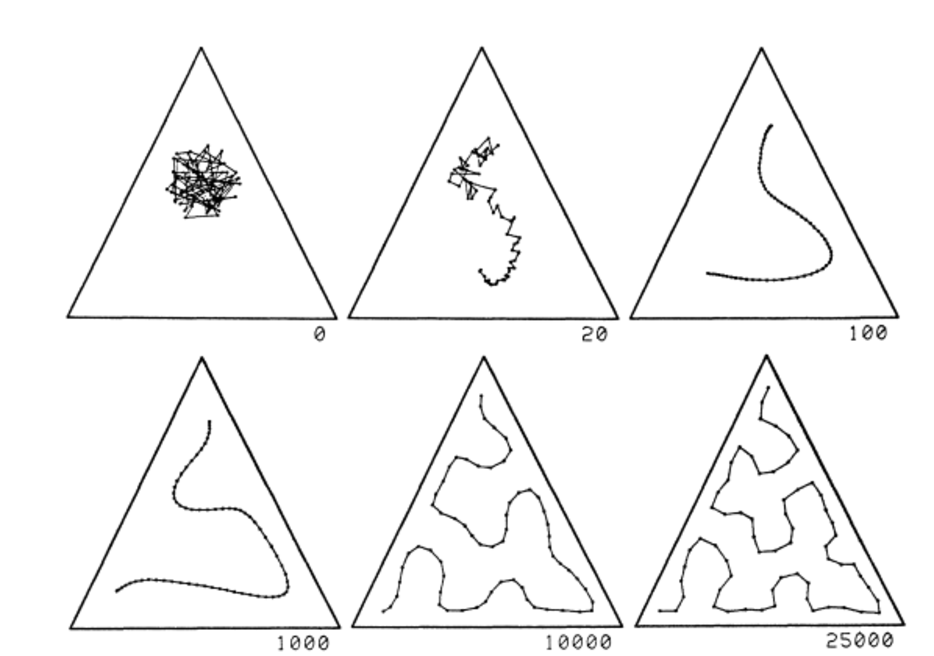
\includegraphics[width=0.7\textwidth]{som1d}
\caption{Dépliement d'une SOM 1D sur des données dans un triangle 2D, tiré de~\cite{Kohonen1995SelfOrganizingM}\label{fig:som1d}}

\end{figure}


\subsection{Inspiration biologique}

% Nous pensons ainsi que les cartes auto-organisatrices sont de bonnes candidates en tant que modules d'une architecture.
% Nous passerons en revue les modèles d'architecture existant en section suivante.
% Avant cela, il est intéressant de s'interroger sur les motivations et les intuitions motivant l'utilisation d'une carte de Kohonen en tant que module d'une architecture.

Le développement des cartes auto-organisatrices par Kohonen est initiallement inspiré par les cartes topologiques observées dans les aires du cerveau. 
Le cerveau est cartographié en \emph{aires corticales} distinctes selon la fonction principale présumée de la zone du cortex correspondante.
Le découpage fonctionnel du cerveau fait apparaître des grandes catégories d'aires corticales. Certaines aires sont dites sensorielles, car elles reçoivent des entrées sensorielles via le thalamus. Certaines aires sont dites motrices et reliées aux muscles, via des structures sous corticales et permettent ainsi un contrôle moteur.
Enfin, des aires sont identifiées comme traitant des informations venant de plusieurs autres aires.
De nombreux travaux montrent la présence de cartes topologiquement ordonnées dans différentes aires du cortex cérébral: les neurones proches dans le substrat cortical réagissent à des stimuli proches. 
Un exemple est ainsi celui du cortex visuel V1, représenté en figure~\ref{fig:v1}. 
L'aire associée à l'audition présente aussi une organisation topographique \cite{Reale1980TonotopicOI}, ainsi que de nombreuses autres aires, directement sensorielles ou plus abstraites \cite{Kohonen1995SelfOrganizingM}. 
Une carte de Kohonen ne doit cependant pas être considérée comme une modélisation biologiquement plausible d'une aire du cortex cérébral, mais plutôt comme une adaptation au niveau computationnel d'un concept biologique, ici le concept d'organisation topologiquement correcte dans les cortex sensoriels, tel que le cortex visuel ou auditif.

\begin{figure}
\centering
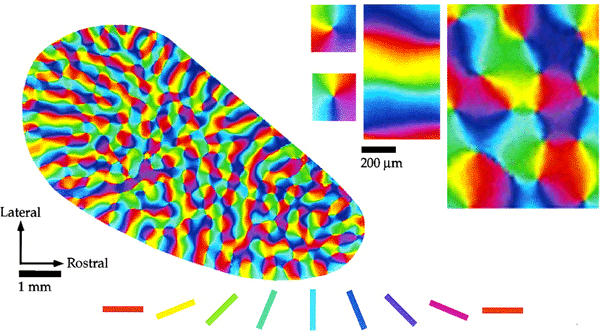
\includegraphics[width=0.6\textwidth]{v1.jpg}
\caption{Représentation des réponses du cortex visuel V1 à un stimulus visuel (bâtonnets d'orientations spatiales différentes). Les neurones répondant à une certaine orientation sont affichés de la même couleur. On observe une continuité entre les neurones proches dans le cortex et l'orientation à laquelle ils répondent. Cette propriété d'organisation est l'inspiration biologique des cartes de Kohonen.}
\label{fig:v1}
\end{figure}


Les aires du cerveau sont connectées entre elles. Notons que cette connectivité du cerveau peut-être étudiée de plusieurs points de vue~: d'un point de vue structurel, en se basant sur des éléments anatomiques ou fonctionnel.
Dans le cas fonctionnel, la connexion de deux aires est déduite de l'existence de dépendances statistiques entre l'activation des neurones des deux aires, observées par éléctroencéphalographie ou IRM fonctionnelle. Il faut noter cependant que ces observations traduisent une relation statistique et pas forcément une relation de cause à effet. 
La modélisation de la connectivité physique de ces aires à partir des observations reste donc l'objet de différentes théories cherchant à reproduire ces corrélations. 
Dans tous les cas, la présence d'aires distinctes communicantes fait l'objet d'un consensus.
Les modèles de base les plus communs pour cette communication entre neurones sont la zone de convergence-divergence de Damasio (CDZ) \cite{damasio_time-locked_1989}, et le modèle de boucles de rée-ntrées de Edelmann \cite{Edelman1982GroupSA}.
La zone de convergence divergence suggère que certaines aires corticales servent d'aires associatives pour associer d'autres zones corticales prenant des modalités sensorielles en entrée. Ces aires associatives assemblent les signaux en provenance des zones sensorielles et les propagent vers d'autres zones. 
La théorie de la ré-entrée postule quant à elle des connexions directes et réciproques entre les neurones de différentes zones sensorielles ou non. Ces connexions sont à l'origine de la coactivation de neurones dans différentes cartes.
% Un tel traitement de l'information permettrait ainsi d'expliquer l'effet ventriloque \cite{Bonath2007NeuralBO}. Lors de cet effet, une activité apparaît dans les cortices visuel et auditif pour les neurones sensibles à l'emplacement exact de la source des stimuli dans chacune des modalités. Après quelques millisecondes, correspondant au temps de trajet de l'aire visuelle à l'aire auditive via les aires associatives, on observe une activité auditive pour les neurones sensibles à l'emplacement spatial de la source du stimulus visuel.

% Le modèle classique du cerveau proposé dans les années 60 [Jones and Powell, 1970] modélise le cortex comme un système de traitement hiérarchique et séquentiel de l'information. Les différents flux sensoriels seraient traités par des aires corticales dédiées, et leur mise en relation dans des aires associatives ui s'occuperaient de tâches de plus haut niveau. 
% Ces flux d'informations circuleraient dans les deux sens: une aire de plus haut niveau recoit des flux d'information montant d'une aire sensorielle, et l'aire sensorielle reçoit des flux d'information descendant des aires associatives. Ce modèle de connexion est par exemple modélisé en \cite{damasio_time-locked_1989}, travaux dans lesquels les zones associatives sont désignées par "zones de convergence-divergence".

% Cette vision hiérarchique historique du traitement cortical de l'information est cependant remise en question par d'autres observations biologiques. Ainsi, \cite{eckert_cross-modal_2008} suggère l'existence de connexions directes entre les aires sensorielles visuelles et auditives. Des théories telles que la réentrée suggère l'existence de neurones multimodaux au sein d'une aire sensorielle. Anatomiquement, de nombreuses connexions, dites bas niveau, entre les aires corticales dédiées au traitement d'une modalité sensorielles ont été mises en évidence chez différentes espèces, pour des aires à différents niveaux hiérarchiques de traitement de l'information(voir [Calvert and Thesen, 2004b, Cappe et al., 2009, Cappe and Barone, 2005, Foxe and Schroeder, 2005, Kayser and Logothetis, 2007, Macaluso, 2006, Schroeder et al., 2003, Schroeder and Foxe, 2005]).
La carte de Kohonen implémentant des concepts computationnels qu'on retrouve en biologie au niveau de l'aire cérébrale, nous pouvons chercher à pousser l'inspiration biologique d'une carte de Kohonen au niveau des connexions entre les aires cérébrales, se transcrivant par des connexions entre plusieurs cartes de Kohonen.
De la même façon qu'une carte n'est pas un modèle biologique, il s'agit plutôt de développer un modèle computationnel qui ne soit pas biologiquement plausible au niveau neuronal, mais dont la structure du traitement de l'information est inspirée de celle du cerveau, ici la présence de plusieurs aires connectées entre elles, modélisées par l'utilisation de plusieurs cartes de Kohonen en architecture.

\section{Architectures de cartes auto-organisatrices}

Plusieurs travaux dans la littérature informatique autour des SOMs cherchent ainsi à construire des architectures de cartes auto-organisatrices. Cette section passe en revue certains modèles.
Nous abordons ces modèles d'un point de vue structurel en s'intéressant notamment à comment s'effectue l'interface entre les cartes dans chacun des modèles. A la lecture des modèles existants, nous avons pu différencier deux grandes classes d'architectures de cartes~: les architectures \emph{hiérarchiques feed-forward} et  les architectures \emph{non-hiérarchiques}, qui peuvent elles-mêmes être \emph{centralisées} ou \emph{décentralisées}.
Nous détaillerons dans cette section ce qu'on appelle architecture hiérarchique et non-hiérarchique et analyserons les comportements d'apprentissage émergeant des différentes structures. L'analyse de ces modèles nous permet de nous situer dans la littérature et d'émettre des hypothèses concernant les comportements attendus d'un tel modèle et ainsi de guider les expériences que nous effectuerons.

\subsection{Architectures hiérarchiques de cartes}

Dès les débuts du développement des SOMs dans les années 1980 des travaux proposent des architectures à base de cartes auto-organisatrices. Ces premiers travaux font apparaître des architectures qu'on peut qualifier de hiérarchiques.
Toutes les architectures hiérarchiques comportent plusieurs cartes, et ont comme point commun qu'il est possible de définir des \emph{niveaux} dans l'architecture, comprenant une ou plusieurs cartes. L'apprentissage des cartes dans toutes ces architectures est effectuée niveau par niveau. Nous les qualifierons ainsi d'architecture \emph{feed-forward}. 

\subsubsection{Architectures hiérarchiques sélectives}

Certains travaux s'appuient sur des architectures hiérarchiques qualifiera de "sélective", dont le principe général est illustrée en figure \ref{fig:hsom_selective}. Toutes les architectures présentées peuvent être séparées en niveaux, dont un niveau d'entrée, un niveau de sortie et des niveaux intermédiaires.
Le premier niveau d'une telle architecture est une carte classique, prenant des données en entrée. 
Après apprentissage du premier niveau, le second niveau est composé de plusieurs cartes.
L'activation ou le BMU de la carte du premier niveau à une entrée permet de sélectionner une carte du deuxième, à laquelle sera présentée cette même entrée. 
Chacune des cartes du deuxième niveau est alors entrainée sur un sous-ensemble des données d'entrée. Pour chaque entrée, la carte à mettre à jour est sélectionnée en fonction de la réponse du premier niveau à l'entrée, d'où
qualification de sélective pour le mode de communications entre cartes~; le premier niveau n'est plus mis à jour lors de cette phase.
Le processus est répété ainsi de suite si besoin sur d'autres niveaux. Les niveaux supérieurs ont alors plus de cartes que les niveaux inférieurs.
Ce procédé est retrouvé dans \cite{barbalho_hierarchical_2001,suganthan_pattern_2001}
\cite{miikkulainen_script_1992} pour de la classification de phrases, \cite{dittenbach_growing_2000,ordonez_hierarchical_2010}, ou encore en \cite{zhao_stacked_2015} pour de la détection d'arrière-plan.

La façon de sélectionner une carte d'un niveau diffèrent ensuite en fonction des travaux.
\cite{barbalho_hierarchical_2001} utilisent la position du BMU calculée au premier niveau pour choisir la carte du second niveau à utiliser. L'architecture utilisée en \cite{zhao_stacked_2015} utilise plusieurs couches de cartes pour du traitement de séquence. Cette fois, le processus de sélection s'opère en choisissant ou non de transférer l'entrée courante au niveau suivant, en s'appuyant sur la distance moyenne de la réponse des cartes à l'entrée.

\begin{figure}
    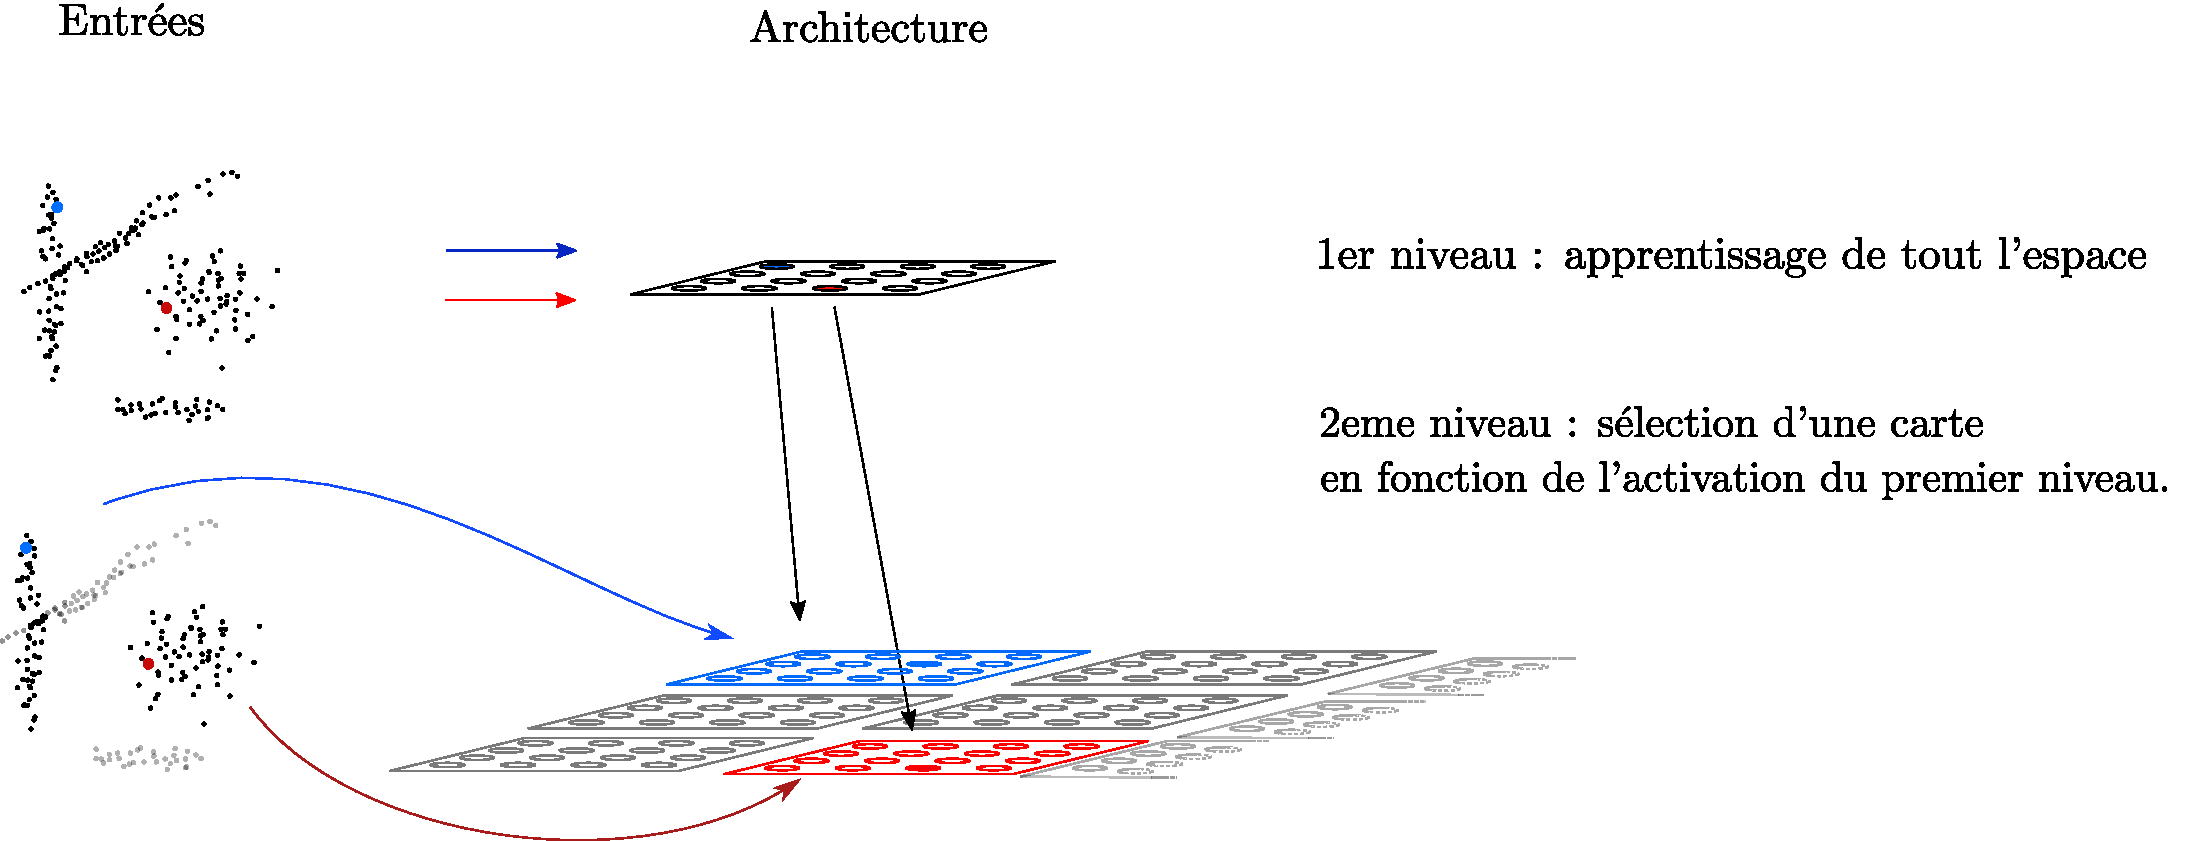
\includegraphics[width=\textwidth]{HSOM_selective.pdf}
    \caption{Exemple d'architecture hiérarchique sélective. La carte du premier niveau est entraînée sur tout l'espace d'entrée. Après apprentissage, la carte permet de filtrer les entrées pour les renvoyer vers une carte du niveau suivant. Dans cet exemple, la position du BMU de la carte du niveau 1 permet de sélectionner une carte du niveau 2, comme c'est le cas en \cite{barbalho_hierarchical_2001}. 
    L'entrée permet d'entraîner une carte du deuxième niveau. Chacune des cartes du niveau 2 apprend alors sur un sous-espace d'entrée.\label{fig:hsom_selective}}
\end{figure}

Dans ce type d'architecture, c'est un processus extérieur aux cartes qui permet de sélectionner la carte du niveau suivant. Les connexions permettent à chacune des cartes de se spécialiser sur une partie de l'espace d'entrée.
Face à ces structures sélectives, on peut imaginer une structure présentant une interface entre cartes qui soit une transmission d'une représentation des données générée par une carte.

\subsubsection{Architectures hiérarchiques par transmission de représentation intermédiaire}

Contrairement aux architectures par sélection, la deuxième couche de carte ne prend plus comme entrée un élément de l'espace d'entrée de l'architecture, mais travaille sur des éléments des cartes des couches précédentes, tels que la position, le poids du BMU ou une intensité d'activité neuronale. 
Ces éléments sont une représentation latente intermédiaire de l'entrée, transmise à la couche supérieure. Les niveaux supérieurs de ce type d'architecture ont moins de cartes que les premiers niveaux et peuvent être considérés comme traitant l'information à un niveau plus abstrait que les cartes du premier niveau.
L'architecture  HSOM \cite{lampinen_clustering_1992} proposée dès 1992 est composée de deux cartes~: une carte apprenant sur des entrées $x$, et une carte prenant comme entrée la position du BMU de la première carte~; cette architecture est illustrée en figure~\ref{fig:hsom}. La position du BMU est ici la représentation intermédiaire transmise aux cartes du niveau suivant.
Comme les cartes s'organisent de façon à conserver les distances dans l'espace d'entrée au sein de la carte, deux éléments faisant partie d'un même groupe de données (cluster) auront des BMUs proches dans la première carte~; par conséquent, leurs BMU dans la seconde carte le seront également. 
Les auteurs notent que l'architecture HSOM permet de bien détecter des clusters de données, avec une séparation des clusters un peu meilleure qu'une SOM classique. La présence de la carte intermédiaire change un peu la façon de séparer les données par rapport à une SOM classique~; les auteurs notent une meilleure séparation des clusters dans HSOM, mais une moins bonne quantification vectorielle au sein d'un cluster. Le fait d'utiliser deux SOMs permet d'extraire une représentation un peu différente que celle extraite par une SOM classique.
Par le choix de la position du BMU comme vecteur de transmission d'information, les auteurs de HSOM exploitent totalement l'aspect topologique qu'offrent les cartes de Kohonen. D'autres travaux par la suite implémentent des modèles similaires transmettant la position du BMU entre cartes, sur des architectures comportant plus de cartes que HSOM, tel que \cite{hagenauer_hierarchical_2013}.
Comme dans les modèles sélectifs, la représentation intermédiaire considérée peut également être les poids des BMUs du premier niveau, comme c'est le cas en \cite{wang_comparisonal_2007, gunes_kayacik_hierarchical_2007}.

On observe un regain de publications sur les architectures de cartes auto-organisatrices après 2015, cette fois sous la terminologie de \emph{Deep SOM}.
La plupart des travaux portant sur ces \emph{Deep SOM} implémentent des cartes hiérarchiques assez similaires aux travaux mentionnés précédemment. 
Mais cette fois, ces travaux s'inspirent des réseaux de neurones profonds (\emph{Deep Learning}), ayant connu leur essor cette même année avec les réseaux convolutionnels permettant l'apprentissage supervisé d'images de façon inégalée \cite{lecun_deep_2015}.
Par analogie avec les réseaux convolutionnels, les Deep SOM s'intéressent souvent à l'apprentissage d'images par des SOMs. Ainsi \cite{Liu2015DeepSM,hankins_somnet_2018,wickramasinghe_deep_2019,aly_deep_2020,sakkari_convolutional_2020,dozono_convolutional_2016,nawaratne_hierarchical_2020-1,mici_self-organizing_2018} et sont présentés comme des "SOMs convolutionnelles". La façon d'associer ces cartes en architectures rappellent cependant les SOMs hiérarchiques.

Par exemple, le modèle introduit en \cite{Liu2015DeepSM} est illustré en figure~\ref{fig:dsom} et s'inspire des réseaux de neurones convolutionnels.
Le but d'une telle architecture est de classifier des images. Une fenêtre est déplacée sur l'image d'entrée et chaque imagette nourrit alors une carte d'une première couche, donnant $N_{maps}  \times N_{maps}$ positions de BMU $j_{p,q}$. Ces positions représentées comme des valeurs en une dimension sont assemblées en une image intermédiaire, chaque pixel prenant la valeur du BMU de la carte correspondante. Une deuxième étape de fenêtrage peut alors être appliquée sur cette image, et ainsi de suite. La dernière couche du réseau est composée d'une SOM qui effectue alors la tache de classification de l'image intermédiaire, vue comme une représentation abstraite  de l'entrée.
L'interface entre les couches "convolutionnelles" est créée à partir des BMUs des SOMs: l'architecture DSOM s'inscrit ainsi directement dans la lignée de HSOM, à la différence qu'un vecteur de positions de BMUs est utilisé comme entrée pour la couche suivante et non la position d'un seul BMU.
Les auteurs montrent que ce modèle est meilleur qu'une SOM classique dans des taches de classification sur MNIST~; les couches supérieures apportent un niveau d'abstraction tandis que les couches inférieures apprennent les motifs.

\begin{figure}
    \centering
    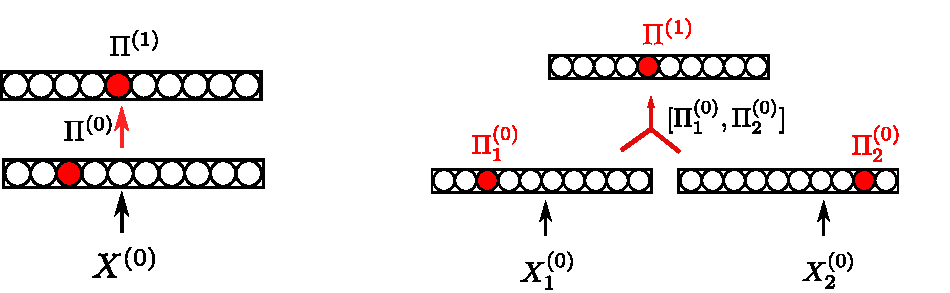
\includegraphics[width=\textwidth]{HSOM.pdf}
    \caption{Architecture HSOM \cite{lampinen_clustering_1992}. L'apprentissage des positions du BMU de la première couche par la seconde permet de mieux détecter les ensembles de données, dans une tâche de clustering. La deuxième couche est vue comme un niveau plus abstrait que la première. \label{fig:hsom}}
\end{figure}

\begin{figure}
    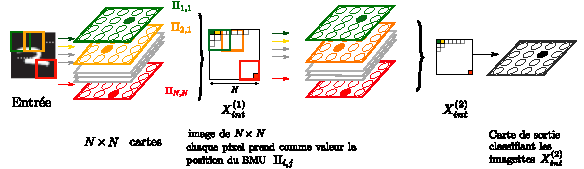
\includegraphics[width=\textwidth]{DSOM.pdf}
    \caption{Architecture DSOM de SOM "convolutionnelle" \cite{liu_deep_2015}. Les auteurs utilisent les positions des BMUs de la couche de carte $j_{p,q}$ comme valeurs d'entrée pour les couches suivantes, dans la lignée de HSOM \cite{lampinen_clustering_1992}. Les couches sont entraînées les unes après les autres. Cette architecture est \emph{feedforward} et \emph{hiérarchique} par transmission de représentation intermédiaire. \label{fig:dsom}}
\end{figure}

Toutes les architectures présentées ici, comme pour les architectures sélectives, sont feed-forward: les couches sont entraînées les unes après les autres. 
Par conséquent, elles ne se prêtent pas à un apprentissage en ligne, tout comme une carte de Kohonen classique.
La plupart des travaux sont appliqués à des tâches de classification qu'on pourrait réaliser avec une SOM classique.
La motivation d'utiliser une architecture plutôt qu'une SOM est alors que la couche finale du réseau possède de meilleures performances en termes de classification que si on avait utilisé une SOM simple.

% Aly ? evoque des perfs similaire à un réseau de deep learning supervisé
% Note : pour une tache de classification, une carte peut eytre comparée à un algo supervisé: la phase de choix de la classe est gérée par un algorithme supervisé après entrainement de la carte.

Nous pouvons conclure de ces travaux qu'il existe différentes façons de transmettre des informations entre couches. Les plus courantes sont la transmission de la position du BMU comme entrée pour la carte suivante, ou un calcul d'activation prenant en compte l'activation de la couche précédente par une connexion neurone à neurone.
La transmission de la position du BMU dans HSOM, Deep SOM et de nombreux autres travaux nous semble particulièrement intéressante car elle exploite totalement l'aspect topologique d'une carte de Kohonen. Par ailleurs, il s'agit d'une valeur de faible dimension, donc se prêtant à des calculs. Les architectures telles que Deep SOM nous montrent qu'une architecture utilisant seulement ce type d'information comme interface est capable de bonnes performances en reconnaissance d'image.
Le champ d'application des architectures feed-forward est le même qu'une SOMs classique~: quantification vectorielle et classification. Leurs performances dans ces domaines surpassent alors celles d'un SOM classique, la présence de couche multiples créant un nouveau niveau d'abstraction.

Nous pouvons donc considérer ces architectures comme des améliorations de carte auto-organisatrices sur des applications spécifiques. Elles n'ont pas la capacité de faire d'autres types de calcul que ceux originalement réalisés dans une SOM.
L'aspect uniquement feed-forward en est la cause: les cartes intermédiaires agissent comme des filtres intermédiaires de l'information donnée en entrée, mais la couche finale reste une carte auto-organisatrice classique.
Cela nous amène à étudier des architectures comportant des boucles de rétroaction~; nous qualifierons ces architectures de non-hiérarchiques. Ces architectures, nous le verrons, permettent de diversifier les comportements d'apprentissage qu'il est possible d'obtenir avec des SOMs en apportant un aspect dynamique au système par les rétroactions.

% C'est l'avenement du deep learning qui a poussé à créer des archi de SOMs. De la meme facon que les réseaux profonds ont étendu les capacités d'apprentissage du perceptron, les couhes de SOM montrent la meme ppté.
% Est-ce que la recherche actuelle sur l'apprentissage non supervisé poussera à remettre les SOM au gout du jour ? Est-ce qu'on ne fait pas de deep som, simplement parce que les outils n'ont pas été développés comme ceux du deep learning ? L'aspect non linéaire d'une SOM peut pourtant etre prometteuse dans ce cadre d'applis.
% Il s'agit par contre d'archiectures completement feed forward: on ne peut pas vraiment parler d'archi modulaires. Les couches sont apprises les unes après les autres.
% On fera référence à ce type d'archis comme des archis hiérarchiques.
% ces arhcitectures montrent des capacités d'apprentissage de motifs à plus grande echelle qu'une carte simple.

% \begin{itemize}
%     \item Historique de l'assemblage des SOMs en architectures feedforward ? 
%     \item Quels sont les avantages apportés par les deep SOMs par rapport à des Soms classiques
%     \item Quels sont les avantages des deep SOM par rapport aux réseaux de deep Learning 
%     \item Pourquoi ne sont elles pas plus utilisées maintenant ?
% \end{itemize}

\subsection{Structures de cartes auto-organisatrices non-hiérarchiques}

Les architectures non-hiérarchiques de SOMs sont des architectures comportant plusieurs cartes communiquant entre elles et dont le schéma de connexion comporte des boucles de rétroaction~: une carte A reçoit de l'information d'une carte B, qui elle-même reçoit de l'information de la carte A.
Ces architectures sont souvent proposées par une motivation d'inspiration biologique, dans le domaine des neurosciences computationnelles, en s'appuyant sur les théories mentionnées précédemment de la réentrée \cite{Edelman1982GroupSA} et des zones de convergence-divergence (CDZ) \cite{damasio_time-locked_1989}.
L'assemblage de réseaux de neurones en architecture fait l'objet de plus nombreux travaux dans le domaine des neurosciences computationnelles. Nous ne détaillerons pas ces travaux ici, nous intéressant spécifiquement aux modèles computationnels destinés à être appliqués en informatique et non modélisant finement la biologie.

Nous avons pu distinguer deux types d'architectures non-hiérarchiques dans l'état de l'art.
Certaines architectures comportent des cartes sensorielles qui sont reliées via des cartes associatives ne prenant pas d'entrées sensorielles, mais seulement des éléments de connexion interne. Ces architectures sont \emph{centralisées} dans la mesure ou ces cartes associatives centralisent l'information  montant des cartes sensorielles et la redistribuent. Ces architectures centralisées sont souvent désignées par leurs auteurs comme hiérarchiques~: en effet, les cartes associatives forment un niveau d'apprentissage différent des cartes sensorielles, apportant une hiérarchie dans l'apprentissage. Nous les classons ici dans la catégorie non-hiérarchique. Bien que des niveaux de cartes peuvent être isolés dans ces architectures, les connexions entre les cartes de deux niveaux sont bidirectionnelles, la carte associative étant à l'origine de l'activation de cartes sensorielles, et réciproquement.
Nous les différencions ainsi des cartes hiérarchiques feed-forward que nous avons listé au paragraphe précédent.
Le second type d'architectures non-hiérarchiques sont celles utilisant des connexions directes entre cartes sensorielles. Ces architectures sont \emph{décentralisées}~: il n'existe pas de module par lequel toute l'information transite.

Un point commun de toutes ces architectures non-hiérarchiques est leur champ d'application~: contrairement aux architectures hiérarchiques feed-forward qui cherchent à améliorer les performances de classification ou de \emph{clustering} d'une SOM classique, les SOM non-hiérarchiques que nous avons relevées dans la littérature sont plutôt appliquées à des tâches de \emph{mémoire associative} sur des données \emph{multimodales}. Ces cartes sont des systèmes dynamiques et ont la capacité de générer une valeur de sortie de façon autonome. Dans la mémoire associative, elles sont alors utilisées pour prédire une modalité à partir d'une autre.

\subsubsection{Architecture comportant une carte associative~: architecture centralisée}

L'idée d'assembler des cartes prenant en entrée une modalité sensorielle par une carte associative a été explorée en \cite{dominey13} et \cite{escobar-juarez_self-organized_2016}.
Dans ces deux travaux de neuroscience computationnelle, les auteurs construisent une architecture se voulant une modélisation du cadre CDZ, mais avec des cartes auto-organisatrices classiques, en transmettant les positions des BMU entre les cartes multimodales. 
Chacune des cartes possède plusieurs couches, chacune prenant une modalité en entrée. Une activité est calculée sur ces modalités en une activité commune. La position du BMU, en l'occurrence un vecteur 3D, sera utilisée comme modalité hiérarchique pour connecter des cartes entre elle. Les auteurs assemblent alors plusieurs cartes sensorielles grâce à des cartes associatives.
Dans le cas d'une hiérarchie de cartes, les auteurs entrainent les couches de l'architecture séparément~: les cartes modales du premier niveau sont apprises, puis la carte amodale les connectant est apprise dans un second temps. 
Une fois toute les cartes apprises, la structure est utilisée pour activer une ou des modalités en activant la carte amodale. Cette carte représente la zone de convergence divergence des modèles cérébraux. 
Dans ce modèle, les cartes sensorielles sont d'abord entraînée, puis les cartes associatives sont apprises dans un second temps. Nous l'avons quand même classée comme non-hiérarchique, car une fois que toutes les connexions sont apprises, elle permet des rétroactions entre cartes. 

Les travaux conduits précédemment dans notre équipe de recherche sur les architectures de cartes auto-organisatrices se classent dans cette catégorie. Ainsi, l'architecture Bijama développée en \cite{menard05,khouzam_2013},associe des cartes modales par une carte associative par des connexions neurone à neurones, en renforçant les connexions entre les groupes de neurones s'activant au même moment dans les cartes modales, via la carte associative.
Notons que Bijama repose sur des calculs complètement locaux, y compris au sein d'une carte auto-organisatrice.



\begin{figure}
    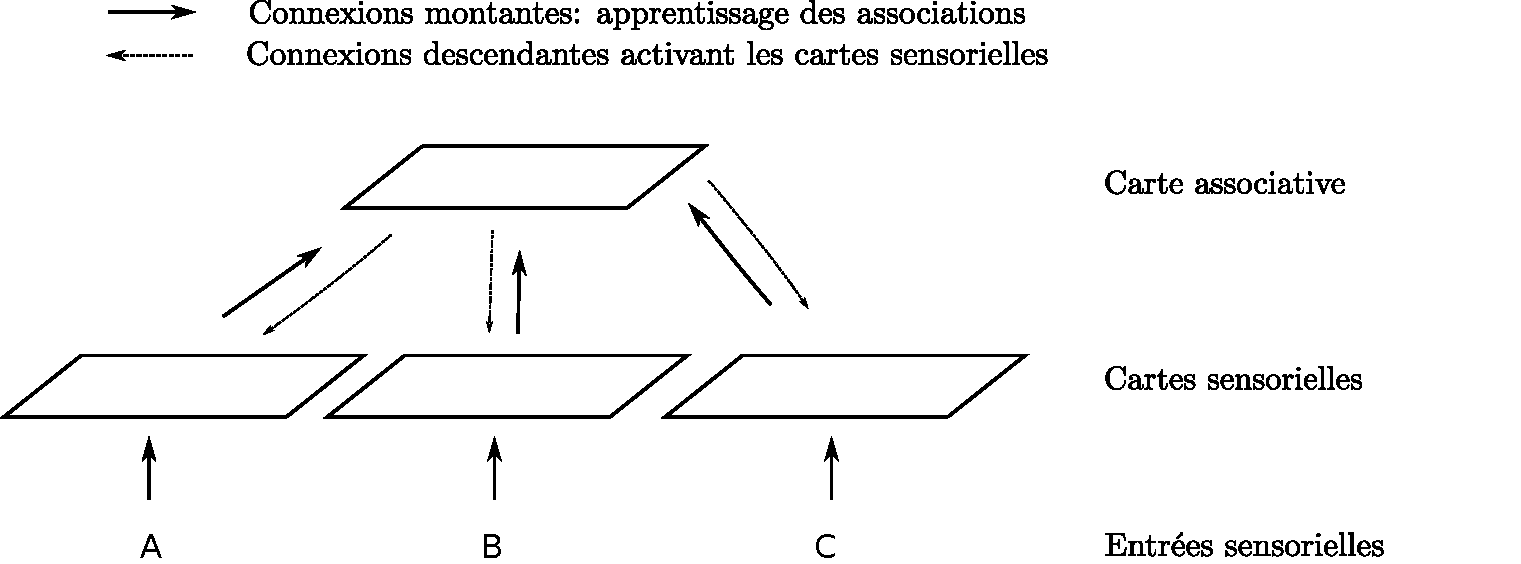
\includegraphics[width=\textwidth]{archi_associative.pdf}
    \caption{Exemple général d'architecture décentralisée comportant une carte associative. Ces architectures sont utilisées dans des tâches de traitement de données multimodales.
     Des cartes appelées cartes \emph{sensorielles} ou \emph{modales} prennent des entrées dans plusieurs modalités. Une carte \emph{associative} reçoit des connexions montantes de ces cartes et apprend à associer les activités. Les cartes sensorielles sont connectées à la carte associative par des connexions descendantes pouvant générer une activation dans la carte. Dans la plupart des modèles, les connexions montantes et descendantes n'ont pas le même rôle: les cartes sensorielles ne s'influencent pas entre elles lors de l'apprentissage.
     Lors de l'utilisation de l'architecture pour de la génération d'entrée sensorielle, alors les connexions descendantes permettent à la carte associative d'activer une carte sensorielle. \label{fig:archi_associative}
     }
\end{figure}

\begin{figure}
    \centering
    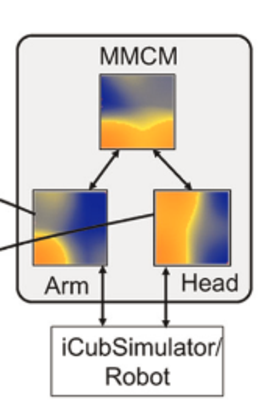
\includegraphics[width=0.3\textwidth]{MMCM_schema.pdf}
    \caption{Architecture MMCM. Les cartes du premier niveau reçoivent l'une les mouvements de tête d'un robot, l'autre les mouvements de main. 
    Une carte amodale (MMCM) reçoit les positions des BMUs de chaque carte du premier niveau. Chaque carte du premier niveau possède également une couche "hiérarchique" prenant en entrée les positions du BMU de MCMM. Chaque niveau est entrainé séparément.
    Après apprentissage, l'activation de la carte MCMM produit des mouvements coordonnés tête/mains~\cite{dominey13}\label{fig:mmcm}}
\end{figure}

Les modèles mentionnés ci-dessus rentrent dans la catégorie non-hiérarchique pour leur possibilité d'activation d'une carte par l'autre. Encore une fois, la position du BMU apparaît chez \cite{dominey13} comme le vecteur de transmission d'information  entre cartes et suffit pour que la coactivation des cartes permettent de réaliser de la mémoire associative. Le modèle SOIMA et le modèle Bijama privilégient la connexion neurone à neurone entre la carte associative et la carte modale, avec une règle d'apprentissage Hebbienne.
Cette mémoire associative est utilisée dans un cadre de données multimodales, avec une notion d'activation d'une carte par l'autre, contrairement aux architectures hiérarchiques citées en section précédentes, utilisées plutot pour des tâches de classification, autrement dit des tâches supervisées.
Dans ces exemples architectures présentées ici, on considère les cartes comme des représentations de leur espace de données qui permettent de la coactivation entres cartes~: une carte de Kohonen prend une fonction générative.

La présence de cartes associatives au sein d'une architecture crée une centralisation de l'information multimodale sur une carte, ce qui nous amène à parler d'apprentissage centralisé. Chaque carte sensorielle ne reçoit aucune information directe d'autres cartes de l'architectures, sauf de la carte associative.

Face aux architectures centralisées, nous pouvons imaginer des architectures décentralisées implémentant des connexions directes entre cartes modales.

\subsubsection{Architectures non-hiérarchiques décentralisées}

Nous avons relevé peu de travaux portant sur des architectures décentralisées, c'est-à-dire comportant des connexions directes entre cartes sensorielles. Un exemple générique d'architecture décentralisée est tracée en figure~\ref{fig:archi_decentralisee}. Les architectures proposées dans tous les travaux que nous avons relevés sont appliquées à de l'apprentissage multimodal.

Une première façon d'associer des cartes de Kohonen est de connecter les neurones d'une carte aux neurones d'une autre par des connexions pondérées. C'est par exemple ce qui est proposé dans \cite{khacef_brain-inspired_2020}. Les auteurs utilisent ici des cartes de Kohonen impulsionnelles, plus directement inspirées de la biologie que les cartes de Kohonen classiques, mais les mêmes principes d'auto-organisation se retrouvent entre les deux modèles. Dans ces travaux, les auteurs apprennent ainsi deux modalités d'un espace multimodale sur deux cartes auto-organisatrices, l'image et le son, puis dans un second temps apprennent les connexions entre neurones en mettant leurs poids à jour à partir des paires d'entrées image-son. Les neurones de chaque carte s'activant sur une même paire d'entrées voient le poids de leur connexion se renforcer, et inversement.
Les auteurs montrent que cette architecture permet d'apprendre les associations d'entrées et peut générer une entrée à partir de l'autre. 
Ce modèle est très simple mais sa mise à jour doit être réalisée en plusieurs étapes~: d'abord les poids des cartes, puis les poids des connexions. Cet apprentissage en deux temps était également présent dans l'architecture centralisée de \cite{dominey13}.

Nous remarquons par contre deux modèles qui cherchent à créer une architecture décentralisée de carte dont l'apprentissage est réalisé d'une seule traite. 

\begin{figure}
    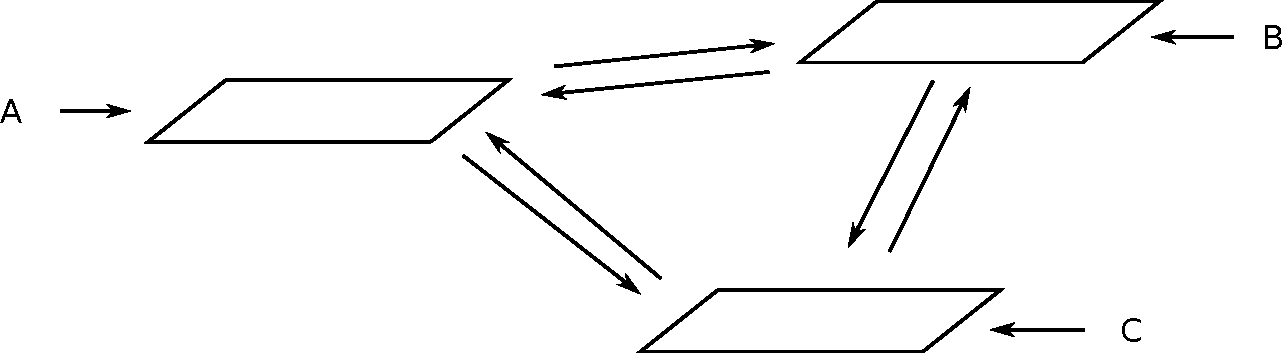
\includegraphics[width=0.9\textwidth]{archi_decentralisee.pdf}
    \caption{Exemple général d'architecture décentralisée de cartes. Chacune des cartes de l'architecture prend une entrée sensorielle A,B,C. Des connexions entre cartes permettent l'apprentissage d'associations entre modalités. Chacune des cartes peut donc être vue comme une carte multimodale. La façon de gérer les rétroactions entre cartes varie en fonction des travaux et est une problématique majeure dans la construction d'une telle architecture. Ainsi, les cartes apprennent à associer leurs activités seulement après avoir appris les modalités en \cite{khacef_brain-inspired_2020} et conjointement en \cite{johnsson_associative_2009} et \cite{baheux_towards_2014}.\label{fig:archi_decentralisee}}
\end{figure}

Une telle version d'architecture de cartes non-hiérarchiques est développée en \cite{johnsson_associating_2008,johnsson_associative_2009}, sous le nom de A-SOM, \emph{associative self-organizing map}. Encore une fois, le but d'une telle architecture est de faire de l'apprentissage multimodal, en apprenant à associer les activités de cartes sur différentes modalités. La particularité de A-SOM, par rapport à tous les modèles précédemment étudiés, est que l'apprentissage de toutes les cartes et de leurs interactions est réalisé simultanément. Ce modèle décentralisé inclut la possibilité de créer une version d'architecture centralisée à partir des règles d'associations, par exemple \cite{buonamente_hierarchies_2016}. Ainsi, un modèle d'architecture décentralisé est intéressant pour la recherche de nouveaux comportements dans la mesure où il n'impose pas de structure spécifique pour l'architecture. La structure des connexions entre cartes devient alors un paramètre sur lequel on peut complètement agir, contrairement aux architectures centralisées.
Une carte du modèle A-SOM possède plusieurs couches de poids. L'une de ces couches est relative à l'entrée de la SOM provenant du capteur. L'autre couche de poids reçoit une entrée provenant d'une autre carte de l'architecture. L'information transmise ici est l'activation de tous les neurones de l'autre carte. chaque carte reçoit ainsi $N\times M$ valeurs d'activité. L'interface entre cartes utilisée en A-SOM est donc le champ d'activation des neurones.

\begin{figure}
    \centering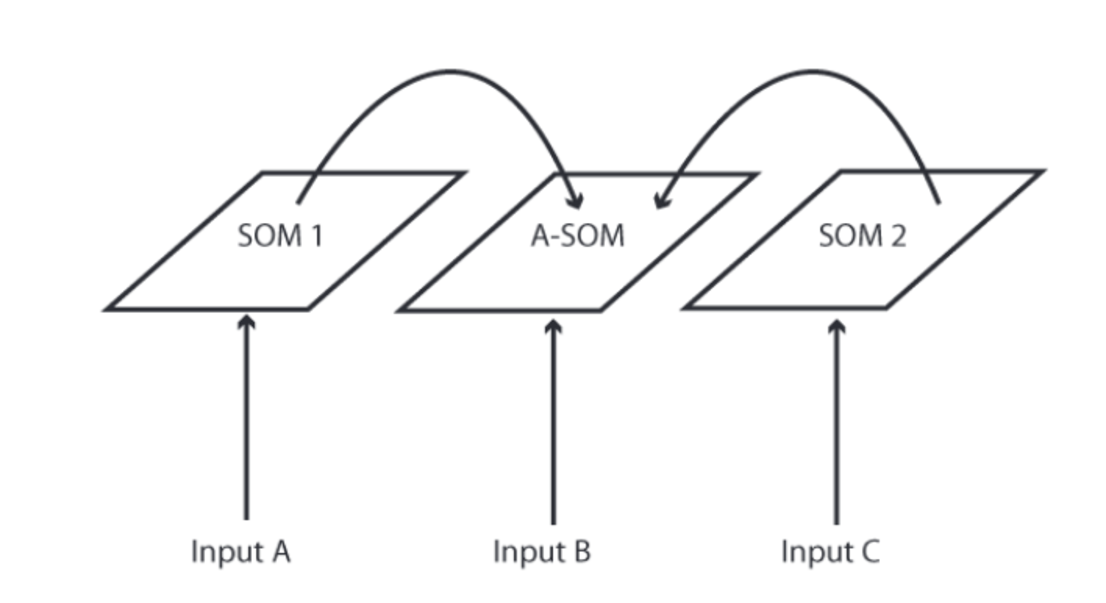
\includegraphics[width=0.7\textwidth]{A-SOM.pdf}
    \caption{Le modèle A-SOM \cite{johnsson_associative_2009} associe les activités de différentes cartes. Chacune des cartes prend une modalité A,B,C en entrée. Contrairement aux modèles précédemment cites, les trois cartes apprennent simultanément. L'association est prise en compte lors du calcul des activités de chaque carte.\label{fig:asom}}
\end{figure}

L'architecture développée en \cite{lefort_active_2015} implémente également une architecture décentralisée pour de l'apprentissage multimodal. De façon similaire à A-SOM, les auteurs associent plusieurs poids aux neurones d'une carte, chacun des poids étant relatif à un type d'entrée~: l'entrée modale et l'entrée venant d'autres cartes. L'information transmise dans ce cas est une partie de l'activité des neurones, celle située dans un carré centré à la même position que le neurone courant. L'information transmise entre cartes est ainsi également un champ d'activation.

\subsubsection{Des modèles multicartes incluant des connexions temporelles}

Certains modèles s'appuient sur plusieurs cartes de Kohonen connectées, en y ajoutant une notion de traitement de séquences.
en \cite{parisiLL}, les auteurs développent une architecture de deux réseaux auto-organisés appelés \emph{grow when required networks} (GWR). Ces réseaux sont des versions incrémentales de cartes de Kohonen dans lesquelles des neurones sont ajoutés au cours de l'apprentissage, le processus de recherche de BMU restant ensuite similaire à une SOM classique.
Cette architecture utilise deux réseaux GWR pour apprendre des séquences, formant une mémoire épisodique et une mémoire sémantique.
La carte associée à la mémoire épisodique (G-EM) est une version récurrente du GWR, dans laquelle des connexions temporelles entre neurones sont mises à jour en supplément des poids associés aux neurones. Le BMU est alors choisi en fonction de l'entrée courante ainsi que des BMUs précédent. 
La deuxième carte est une version classique du GWR. Elle prend en entrée une séquence de BMUs de la carte G-EM, ainsi que la classe de la séquence courante, afin de mettre à jour ses poids. 
Cette architecture associe ainsi des connexions temporelles récurrentes sur une carte ainsi que des connexions entre cartes.
Cette architecture permet des tâches de \emph{lifelong learning}. 
Le concept d'apprentissage sur le long terme s'intéresse à des systèmes étant mis à jour en ligne, dès qu'ils recoivent une entrée, et dont l'apprentissage n'a pas de limite temporelle fixé. On doit donc avoir un système qui trouve de lui-même une stabilité dans l'apprentissage et qui est capable de s'adapter à de nouvelles entrées.
Dans la plupart des applications en robotique, les entrées présentées à une structure d'apprentissage sont par ailleurs des entrées ayant une relation temporelle. Deux images recues successivement par un capteur visuel seront proches dans l'espace des images. Pour une SOM par exemple, cela pose problème. Les archcitectures de lifelong learning cherchent donc une solution à ces problèmes pour créer une structure autonome, évoluant dans le temps et permettant de réaliser la tâche pour laquelle elle est conçue tout en continuant à être mise à jour, sans oublier les données vues au début de l'apprentissage.
Les auteurs utilisent leur architecture pour de la reconnaissance d'objets. Cependant, lors de l'apprentissage, les données ne sont pas présentées après un tirage aléatoire dans l'espace, mais sont présentés classe par classe~: tous les objets d'une même classe d'abord, etc. Les auteurs montrent que l'architecture est capable de bien prédire la classe d'un objet lors d'un test sur toutes les classes apprises. \`{A} titre de comparaison, une SOM classique apprendrait la classe du premier objet, puis l'oublierait pour se déplier entièrement sur la deuxième classe, etc. A terme, seule la dernière classe apprise est gardée en mémoire.

La motivation de ces modèles multicartes est intéressante~: il s'agit cette fois de voir les deux cartes comme de l'apprentissage à différentes échelles temporelles. L'architecture mélange connexions récurrentes et connexions inter-cartes, ce qui est pertinent dans le cadre de l'apprentissage de séquence, et dans le but de création de systèmes autonomes de cartes auto-organisatrices évoquées par Kohonen. 
Cependant, si sa motivation nous intéresse, le modèle décrit précédemment utilise une logique de vérification externe aux cartes pour ajouter ou nom des neurones. 

Notre démarche s'inscrit dans un objectif d'allier connexions temporelles et connexions intercartes au sein d'une même architecture, sans forcément avoir à différencier ces connexions.
Les travaux autour du modèle A-SOM mentionné précédemment en ont ainsi dérivé une version récurrente \cite{Buonamente2015DiscriminatingAS}. Cette version récurrente est similaire à la version multicarte. Au lieu de considérer l'activité d'une autre carte pour le calcul de l'activité courante d'une carte, les auteurs utilisent l'activité de la même carte à l'état précédent.
Cette structure est appliquée à la prédiction de mouvement. De la même façon qu'une architecture est capable, à partir d'une modalité, de prédire les valeurs correspondant à l'autre modalité, l'architecture incluant une version récurrente peut prédire la fin d'une séquence à partir de son début. La motivation de développer une version récurrente de A-SOM est alors de pouvoir développer des architectures comportant connexions récurrente et connexions intercartes. Nous n'avons pas encore relevé cependant de travaux les intégrant effectivement dans une architecture multicartes.

Les travaux menés en \cite{baheux_towards_2014} ont également cherché à insérer des connexions temporelles au sein d'une architecture de deux cartes, présentée en \ref{fig:baheux}. Chaque carte est composée de deux couches de poids. Une des cartes prend une entrée correspondant à l'observation courante, relative à une première couche de poids, comme une SOM classique. La deuxième couche de poids est relative à l'information interne descendant de la seconde carte, qui est la position du BMU de la deuxième carte. 
La seconde carte recoit deux entrées de la première~: une entrée est la position du BMU de l'état précédent et la seconde la position du BMU de l'état courant. Une activité est calculée sur chaque couche de poids relativement à son entrée et ces deux activités sont fusionnées en une activité globale à chaque carte.
Comme chaque carte reçoit en entrée la position de l'état courant du BMU de l'autre carte, il existe une boucle de rétroaction entre carte. Les auteurs laissent alors "résonner" les activités en déplacement petit à petit les BMUs de chaque carte, jusqu'à obtenir un état stable pour les activités, qui est utilisé pour déterminer le BMU final servant à la mise à jour des poids. 
Ce modèle permet alors d'apprendre des séquences d'entrée. Alors qu'une carte simple différencierait les BMUs en fonction de la valeur de l'entrée, ce modèle génère une différenciation des BMUs en fonction de la position d'un élément dans la séquence en plus de sa valeur. 


\begin{figure}
    \centering
    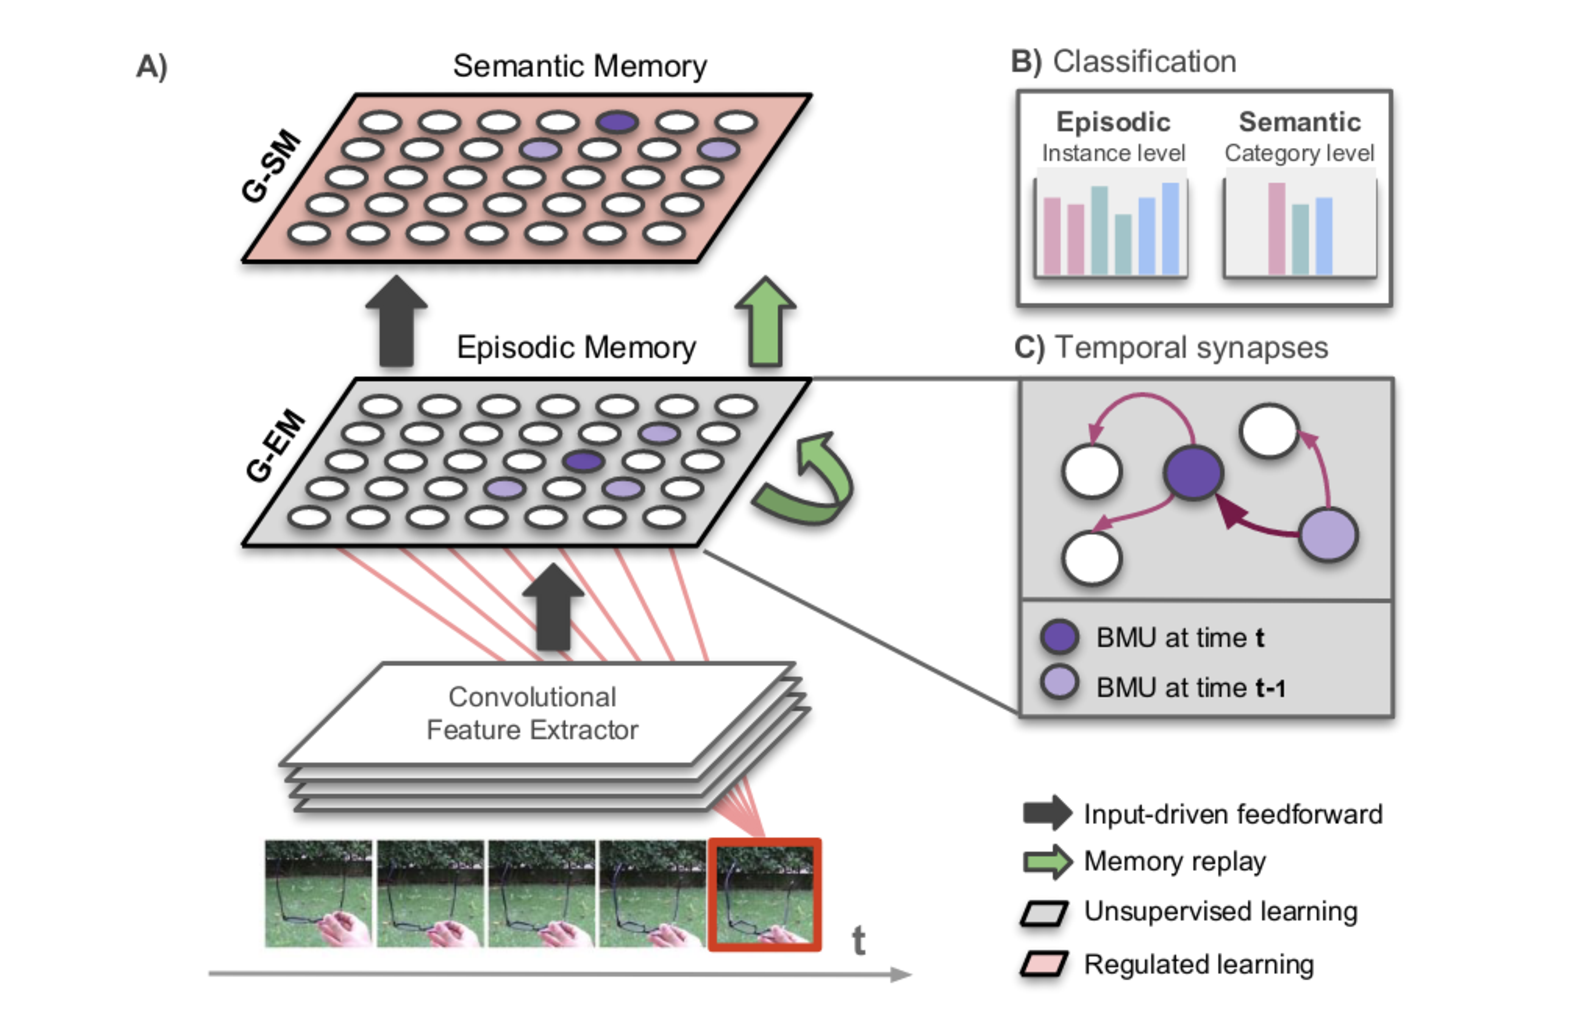
\includegraphics[width=0.8\textwidth]{Parisi_2020.pdf}
    \caption{Architecture \emph{à double mémoire} proposée en \cite{parisiLL}. La couche de mémoire épisodique est un réseau \emph{grow when required (GWR)}, un réseau auto-organisé similaire à une carte de Kohonen, à la différence que les neurones sont ajoutés au fur et à mesure de l'apprentissage. La couche de mémoire sémantique est également un réseau GWR, entraîné à partir des BMUs de la couche épisodique et de la classe de la séquence jouée. L'architecture apprend à reconnaitre plusieurs séquences.\label{fig:gdm_parisi}}
\end{figure}

\begin{figure}
    \centering
    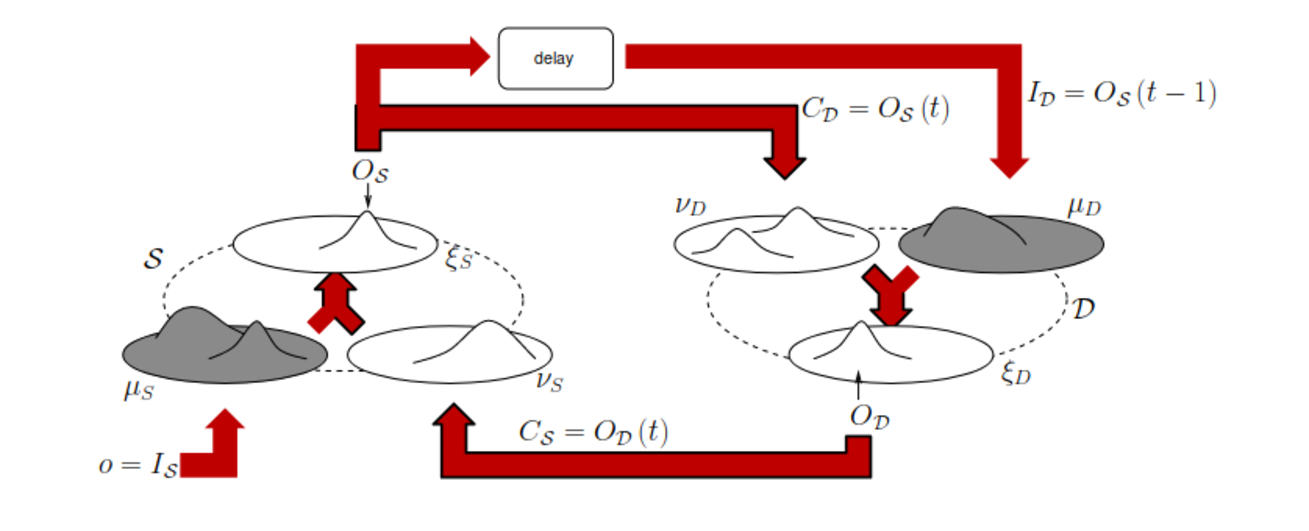
\includegraphics[width=0.8\textwidth]{baheux.pdf}
    \caption{Structures de deux cartes auto-organisatrices communicantes, \cite{baheux_towards_2014}. Chaque carte est composée de trois couches d'activités, représentées séparément sur le schéma: sur la première carte, une activité est relative à l'entrée $o$, l'observation. L'autre activité reçoit une entrée descendant de la seconde carte. Ces deux activités sont fusionnées en une activité globale servant à déterminer un BMU. La seconde carte reçoit ensuite deux entrées venant de la première carte : le BMU de l'état courant et le BMU de l'état précédent. Un système de résonnance est mis en place pour gérer les boucles de rétroactions entre BMUs, comme chaque carte reçoit le BMU de l'état courant de l'autre carte en entrée. Ce principe laisse évoluer dynamiquement les activités vers un état stable, utilisé ensuite pour la détermination du BMU final.\label{fig:baheux}}
\end{figure}

Ces exemples nous amènent à pousser la bibliographie de cette thèse sur les cartes de Kohonen récurrentes. On voit en effet la similarité existant dans le traitement de séquences, ou le choix d'un BMU doit prendre en compte le contexte des états précédents, aux modèles multimodals dans lequel le choix d'un BMU doit prendre en compte le contexte des entrées d'autres modalités. 

\subsection{Cartes auto-organisatrices récurrentes}

\begin{figure}
   \centering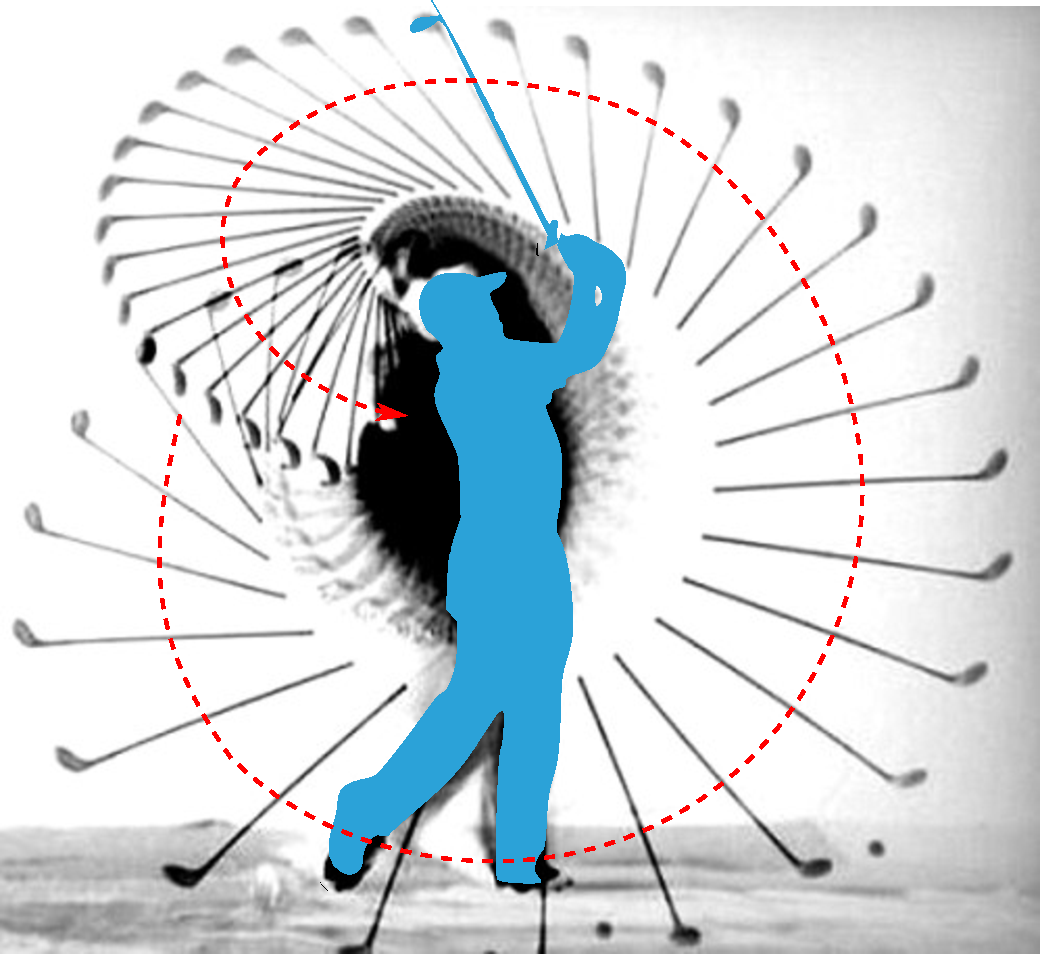
\includegraphics[width=0.6\textwidth]{movment_002.pdf}
   \caption{L'image présentée à un réseau (en bleu) correspond à un instant d'une séquence. L'objectif de l'apprentissage non-supervisé de séquences est d'extraire une représentation d'une séquence d'entrée. Une utilisation commune est la classification de mouvements. La séquence "tirer" sera différente de la séquence "marcher".\label{fig:mouvement}}
\end{figure}

On appelle réseaux récurrents des réseaux de neurones qui prennent en compte leur état précédent pour calculer leur état actuel. Ces réseaux sont utilisés pour le traitement et l'apprentissage de signaux temporels. Citons par exemple, en Deep Learning, les RNN (\emph{recurrent neural networks}), dont les neurones reçoivent leur état précédent en entrée. Les cartes de Kohonen ont ainsi également des versions récurrentes.

Nous nous intéressons aux architectures multicartes, mais les cartes récurrentes répondent à des problèmes très similaire à ceux rencontrés dans la conception d'architectures de cartes pour faire de la mémoire associative, comme vu en section précédente.
Dans une carte récurrente, le problème principal est de trouver comment communiquer à la carte de l'information sur son état précédent et comment utiliser cette information dans l'apprentissage de l'état courant. Cela rejoint la problématique posée dans les architectures de cartes de Kohonen, qui est de comment communiquer à une autre carte son état, afin de l'utiliser dans l'apprentissage de l'état courant. L'étude des modèles de cartes récurrentes existant nous permettrons de compléter cette bibliographie. 

Notre volonté de créer un modèle général d'architecture de cartes auto-organisatrice motive également le fait de s'intéresser aux cartes récurrentes. On souhaite en effet créer un modèle qui puisse unir cartes récurrentes et cartes normales au sein d'une même architecture. L'aspect bio-inspiré du modèle et son aspect multimodal ciblent plutot des applications d'un tel réseau en robotique. Or, la plupart des données traitées par des réseaux de neurones, en particulier dans les applications robotiques, sont temporelles : vidéos, signaux sonores, capteurs de position. Il est donc important de s'appuyer autant sur les modèles de cartes récurrentes existantes que sur les architectures afin de créer un modèle général.

Les modèles de cartes récurrentes existant dans la littérature se classent en catégories similaires aux modèles multicartes que nous avons listé.
D'une part, certains modèles de cartes utilisent l'état précédent de la carte lors du calcul de \emph{l'activité} de l'état courant. De l'autre, des modèles réutilisent plutôt des éléments de la carte à l'instant précédent directement en tant qu'\emph{entrée} de l'état courant.


Parmi les premiers travaux autour des cartes auto-organisatrices, l'Hypermap \cite{Kohonen1991THEHA}, dérivée ensuite en \emph{recurrent SOM} \cite{varsta_temporal_2001} conditionnent la recherche de BMU d'une carte à un contexte dépendant de l'état précédent, lié à l'entrée précédente dans la séquence. Ce contexte repose sur la limitation d'une zone de la carte dans laquelle faire la recherche du BMU. 

D'autres travaux reposent sur la transmission d'un contexte en tant qu'entrée complétant l'entrée courante. 
Ainsi, les \emph{recursive SOMs} de \cite{Voegtlin2002RecursiveSM} prennent deux entrées~: l'élément de la séquence ainsi qu'un vecteur contenant l'ensemble des activations des neurones de la carte à l'état précédent.
MSOM, de \cite{Strickert2005MergeSF} s'appuie sur le poids du BMU. A chaque instant, l'entrée de contexte à transmettre à l'état suivant est définie comme une combinaison linéaire entre le poids du BMU courant et le contexte courant.
Le modèle SOMSD \cite{hagenbuchner_self-organizing_2003, hammer_recursive_2004,hammer_self-organizing_2005, fix20} réduit ce contexte à la position de la Best Matching Unit.
Les travaux de \cite{Buonamente2013SimulatingAW} proposent une version récurrente du modèle A-SOM présenté en section précédente. Le contexte considéré est alors un ensemble d'activités de neurones.
Les mécanismes de transmission de contexte entre instants dans les cartes récurrentes s'appuient sur les mêmes mécanismes que ceux proposé dans le cadre d'architectures de cartes~: sélection de région de la carte, transmission d'activation, et enfin transmission du BMU.
Les travaux menés en \cite{fix20} sur le modèle SOMSD montrent qu'une carte récurrente parvient à différencier ses BMUs en fonction de la position de l'entrée dans une séquence et non seulement de la valeur de l'entrée.

\section{Axe de recherche}

Nous avons détaillé la littérature existante en terme d'architecture de SOMs et plus généralement de réseaux de neurones auto-organisés. Nous avons divisé ces architectures en deux grandes catégories~: un format hiérarchique et \emph{feedforward}, et un format non-hiérarchique incluant des rétroactions.
Le format feed forward implique généralement un apprentissage couche par couche. Ce format est très appliqué et permet d'améliorer les capacités de clustering d'une SOM classique, principalement dans le cas ou les données traitées présentent elles-mêmes une structure hiérarchique, telles que des images ou des phrases.
Nous cherchons à développer une architecture plus générale de cartes auto-organisatrices et ne nous placons ainsi pas dans le contexte des Deep SOM mentionné ci-dessus. 
Cependant, nous notons que la position du BMU comme interface entre couche de cartes permet des capacités de calcul.
Nombre de ces architectures sont développées directement dans un but applicatif. On peut ainsi faire la distinction entre un modèle d'architecture, tel que HSOM, qui est générique et applicable à tout type de données, et une structure appliquée, développées spécifiquement pour un type de données.

Opposées à ces architectures hiérarchiques, des architectures reposent sur de l'interaction entre cartes, avec des boucles de rétroaction.
Ces architectures sont moins présentes dans la littérature que les Deep SOM, et cherchent en général à se rapprocher d'un contexte biologique.
Nous nous plaçons plutôt dans la lignée des cartes non-hiérarchiques, sans vouloir cependant copier un aspect biologique.
De façon intéressante, nous remarquons que plusieurs structures non-hiérarchiques sont associées à l'apprentissage de données temporelles. Ces architectures se rapprochent des modèles appelés cartes auto-organisatrices récurrentes, dans lesquels des éléments de calcul d'une carte à une itération données sont réutilisés pour le calcul des itérations suivantes.
Ces architectures non-hiérarchiques dynamiques se divisent en architectures centralisées et décentralisées. La décentralisation des calculs va dans un sens de l'informatique non conventionnelle.

Ces modèles soulèvent également une problématique dans les algorithmes d'apprentissage d'architecture non-hiérarchiques comportant des rétroactions. Dans le cas des neurones impulsionnels, les impulsions des neurones arrivent en différé, une connexion réciproque entre neurones ne pose pas de problème~: les neurones sont traités dans l'ordre des impulsions. Dans le cas de cartes de Kohonen, qui ne repose pas sur des séries d'impulsions, l'information arrive simultanément dans les différentes cartes. L'activité de la carte A influence l'activité de la carte B, mais l'activité de la carte B influence également celle de la carte A, formant une boucle de rétroaction potentiellement infinie. Les architectures mentionnées font le choix d'apprendre d'abord les cartes sensorielles de façon indépendante, puis d'apprendre seulement leurs connexions dans un second temps, décomposant ainsi la boucle. 
La rétroaction est ensuite utilisée en phase applicative pour générer une modalité~: seule une des cartes sensorielle prend une entrée, l'autre carte est considérée comme la sortie de l'architecture et réagit à l'activité des autres cartes. Les rétro-actions ne sont alors pas non plus un problème en phase d'application.

Notons enfin que limites entre les catégories d'architectures que nous avons différenciées dans ce chapitre sont floues. Une architecture décentralisée peut contenir des sous-structures hiérarchiques ou au contraire, une structure hiérarchique de modules décentralisés peut être imaginée.

Parmi ces axes de développement d'architectures, nous choisissons de nous intéresser dans cette thèse à des architectures non-hiérarchiques de cartes.
Les architectures hiérarchiques nous paraissent de bonnes candidates à améliorer les performances d'une SOM sur une application spécifique comme du traitement d'images, tandis que les architectures non-hiérarchiques offrent de nouvelles possibilités de calcul, non envisageables par des SOM classiques, telles que la génération d'entrée, et c'est cet axe que nous souhaitons explorer.
%L'observation d'émergence de calcul dans des systèmes complexes d'apprentissage, introduite au chapitre~\ref{chap:modularite} vient appuyer ce concept.
Peu de travaux ont par ailleurs exploré l'idée d'associer des SOMs en architectures comportant des rétroactions.
Les choix pour la construction d'une telle architecture se situent au niveau de l'interface entre cartes. De nombreux travaux autour des cartes de Kohonen utilisent la position du BMU comme vecteur de l'information transmise entre plusieurs cartes. 
Nous faisons ce choix également. Il apparaît comme une valeur peu coûteuse à communiquer entre cartes, mais qui contient beaucoup d'information sur l'état d'une carte. Cette valeur se présente également comme un cadre homogène de communication intercarte: quelles que soient les entrées sur lesquelles apprend une carte, il sera toujours possible de la connecter à d'autres cartes de l'architecture. 
Enfin, on retrouve l'utilisation de la position du BMU à la fois dans des architectures multicartes et dans les cartes récurrentes comme SOMSD. Le cadre choisi permettrait donc d'intégrer à la fois des cartes classiques et des cartes récurrentes au sein d'une même architecture, offrant encore plus de possibilités de calcul.
Ce modèle de connexions par transmission de position de BMU n'a pas été exploré pour créer des architectures non-hiérarchiques décentralisées. Cette thèse se veut l'exploration de ce modèle.
Nos travaux font ainsi suite à \cite{baheux_towards_2014} sur des architectures récurrentes multimodales utilisant la transmission de la postion du BMU entre des cartes de Kohonen, exploitant la position du BMU comme les travaux sur les cartes récurrentes SOMSD \cite{hagenbuchner_self-organizing_2003,Strickert2003UnsupervisedRS,fix20}.
Les travaux commencés en \cite{baheux_towards_2014}, bien qu'ils exploitent des connexions intercartes, sont similaires à ce qu'on obtiendrait avec une carte récurrente simple, telle que celle décrite en \cite{fix20}.
Nous voulons continuer sur le même modèle, utilisant la transmission du BMU, qui nous apparaît comme une solution compacte et facilement extensible à grande échelle pour construire des grandes architectures, mais en explorant cette fois l'aspect des connexions intercartes.
Par leur motivation, qui est le développement d'un système multi-som, nos travaux se rapprochent aussi des travaux conduits sur l'architecture A-SOM \cite{johnsson_associating_2008, johnsson_associative_2009,gil_sarasom_2015, Buonamente2015DiscriminatingAS}~; notre modèle de carte et d'interface est par contre différent.



\begin{figure*}[b]
    \centering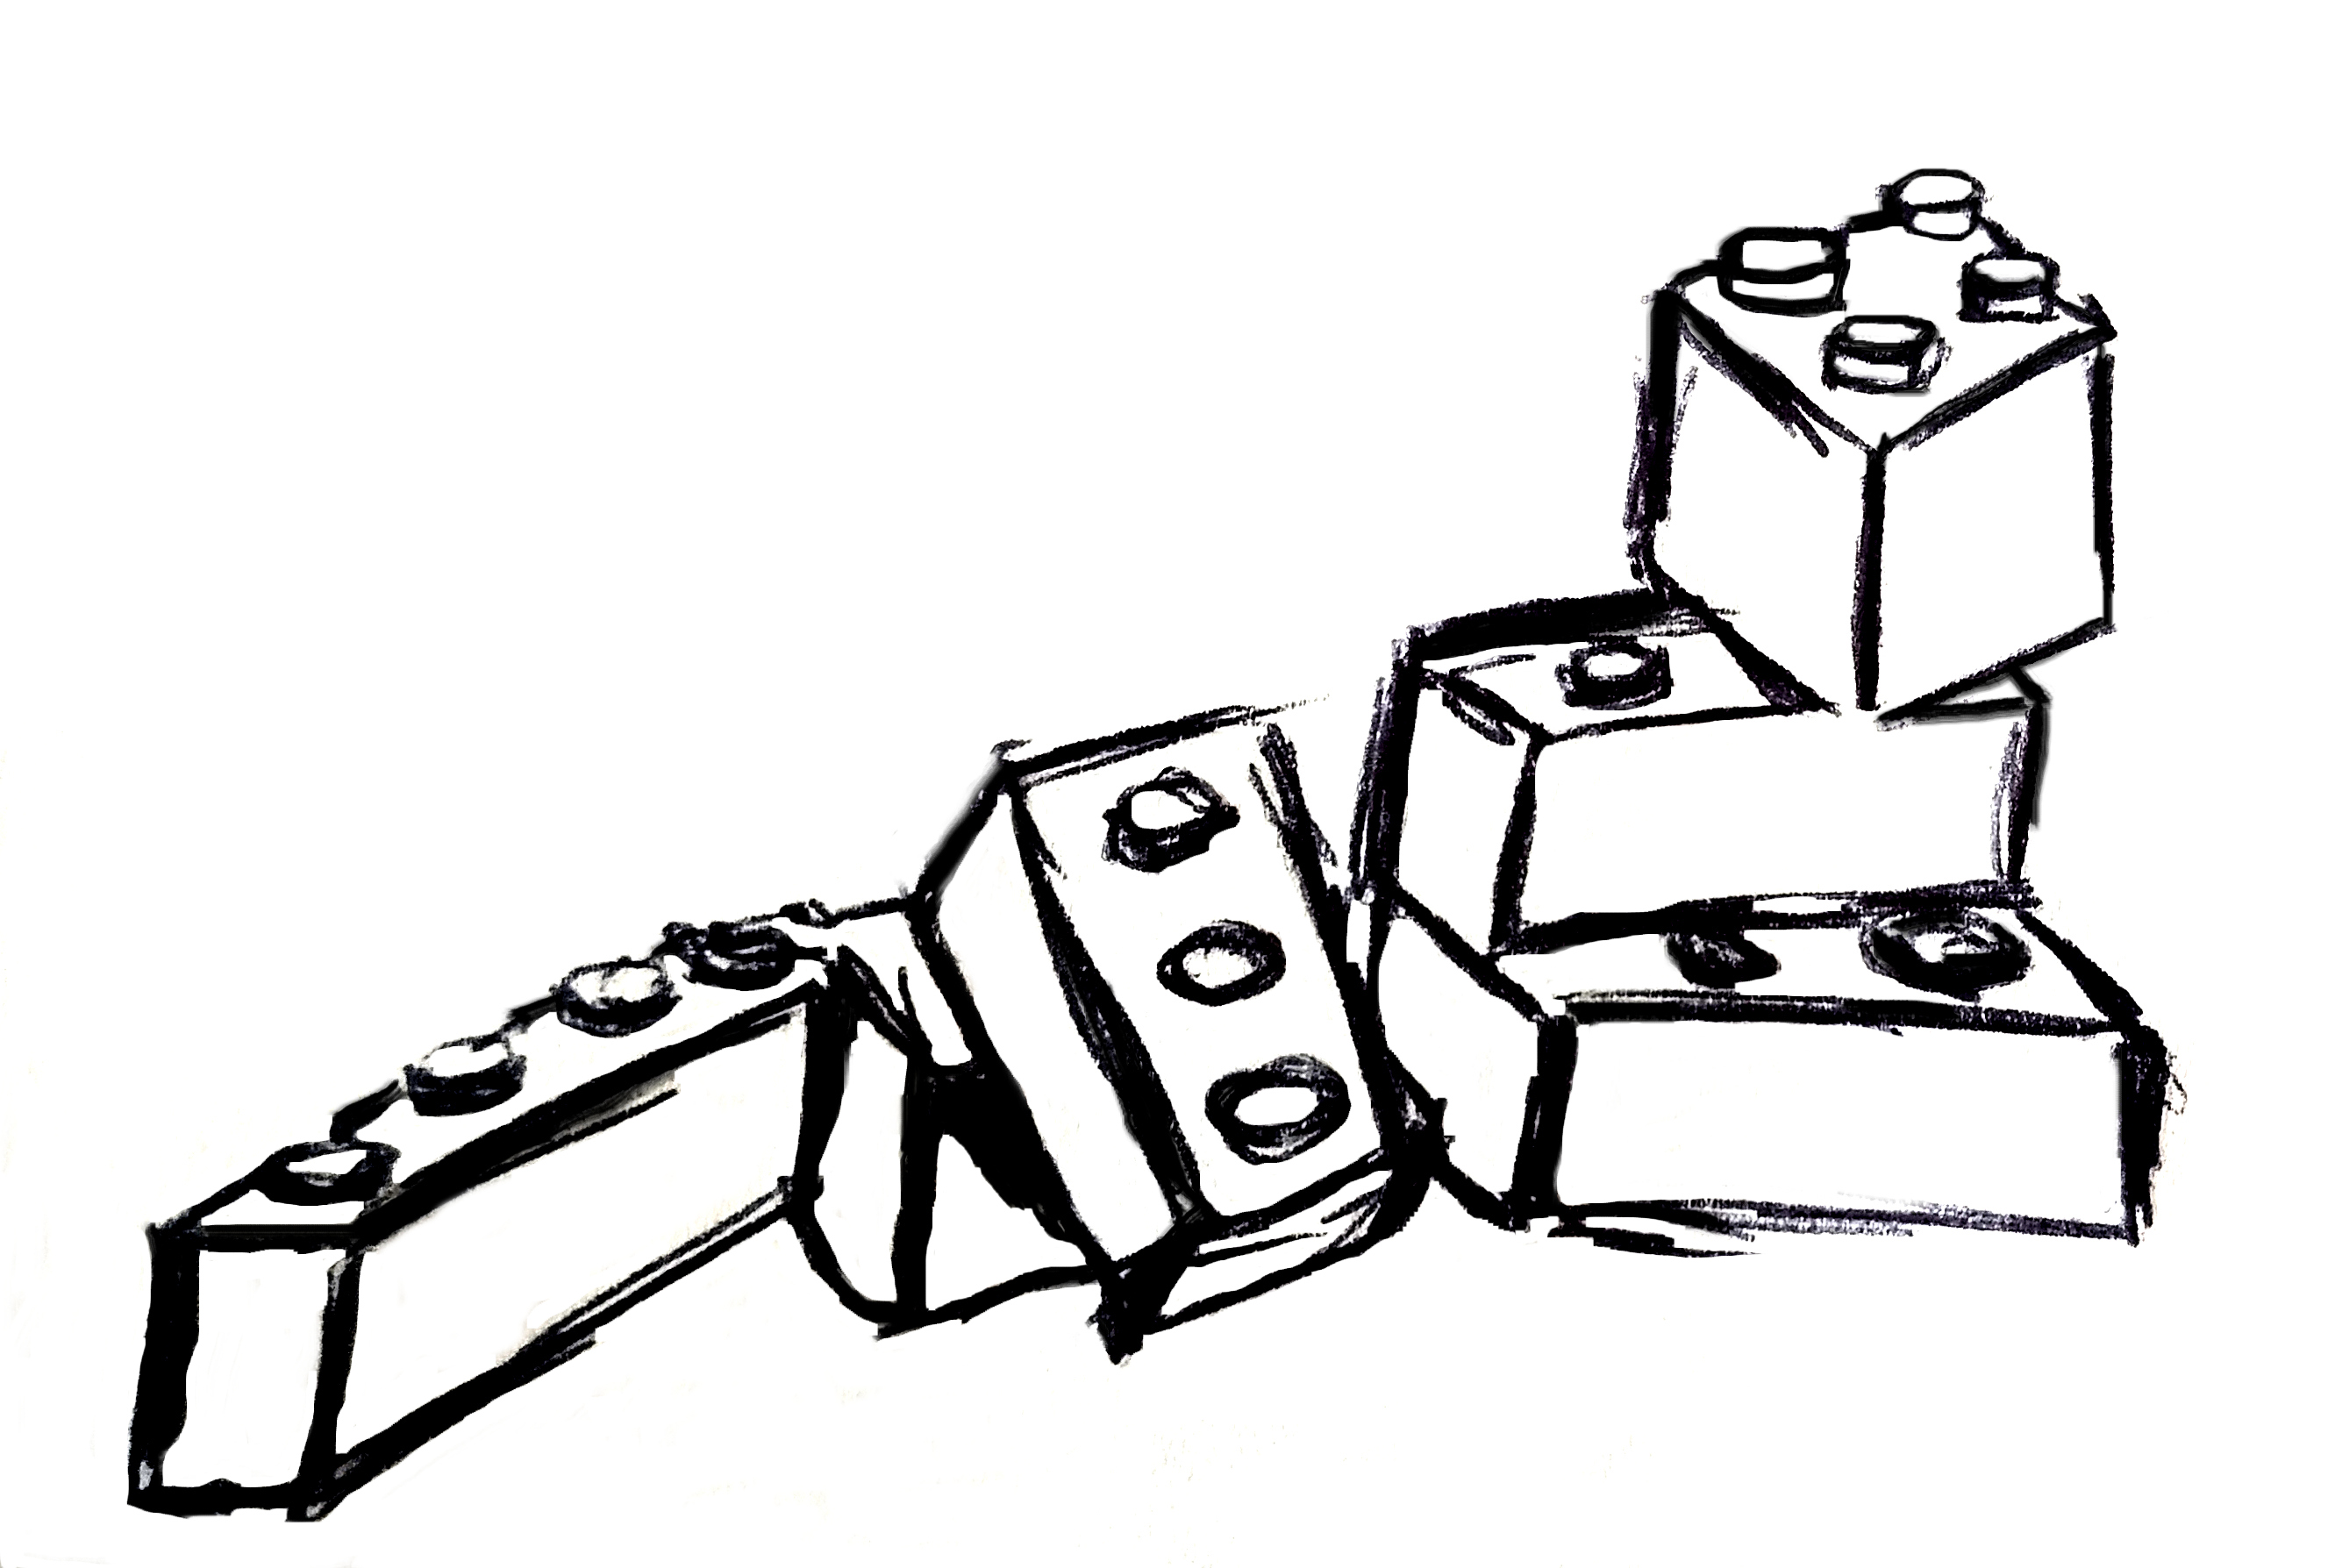
\includegraphics[width=0.6\textwidth]{lego2.jpg}
\end{figure*}

\ifSubfilesClassLoaded{
    \printbibliography
    %\externaldocument{../main.tex}   
}{}
\end{document}